\documentclass[compress, aspectratio=169]{beamer}


\usetheme{Frankfurt}
\setbeamertemplate{page number in head/foot}[totalframenumber]

%% UNBC Color Theme
\definecolor{UNBCGreen}{RGB}{3,86,66}
\definecolor{UNBCGold}{RGB}{183,149,39}
\setbeamercolor{alerted text}{fg=UNBCGold}
\setbeamercolor{background canvas}{bg=white}
\setbeamercolor{block body alerted}{bg=normal text.bg!90!black}
\setbeamercolor{block body}{bg=normal text.bg!90!black}
\setbeamercolor{block body example}{bg=normal text.bg!90!black}
\setbeamercolor{block title alerted}{use={normal text,alerted text},fg=alerted text.fg!75!normal text.fg,bg=normal text.bg!75!black}
\setbeamercolor{block title}{bg=white}
\setbeamercolor{block title example}{use={normal text,example text},fg=example text.fg!75!normal text.fg,bg=normal text.bg!75!black}
\setbeamercolor{fine separation line}{}
\setbeamercolor{frametitle}{fg=white}
\setbeamercolor{item projected}{fg=white}
\setbeamercolor{normal text}{bg=black,fg=black}
\setbeamercolor{palette sidebar primary}{use=normal text,fg=normal text.fg}
\setbeamercolor{palette sidebar quaternary}{use=structure,fg=structure.fg}
\setbeamercolor{palette sidebar secondary}{use=structure,fg=structure.fg}
\setbeamercolor{palette sidebar tertiary}{use=normal text,fg=normal text.fg}
\setbeamercolor{section in sidebar}{fg=UNBCGold}
\setbeamercolor{section in sidebar shaded}{fg=grey}
\setbeamercolor{separation line}{}
\setbeamercolor{sidebar}{bg=white}
\setbeamercolor{sidebar}{parent=palette primary}
\setbeamercolor{structure}{bg=black, fg=UNBCGreen}
\setbeamercolor{section in toc}{fg=white, bg=white}

\setbeamercolor{subsection in sidebar}{fg=UNBCGold, bg=UNBCGold}
\setbeamercolor{subsection in sidebar shaded}{fg=UNBCGold, bg=UNBCGold}
\setbeamercolor{subsection in sidebar highlighted}{fg=UNBCGold, bg=UNBCGold}
\setbeamercolor{title}{fg=white}
\setbeamercolor{titlelike}{fg=blue}
%%%

%% Change shape of bullets
\setbeamertemplate{itemize items}[circle]
\setbeamertemplate{enumerate items}[circle]
%%%

%% Import packages
\usepackage{array}
\usepackage{booktabs}
\usepackage{tcolorbox}
\usepackage{graphicx}
\usepackage{xcolor}
\usepackage{colortbl}
\usepackage{amsmath}
\usepackage{pifont}
\usepackage{ccicons}
\usepackage{tikz}
\usepackage{tikzlings}
\usetikzlibrary{mindmap}
\usepackage{smartdiagram}
\usepackage[linesnumbered,lined,commentsnumbered]{algorithm2e}
\usepackage{hyperref}
\tcbuselibrary{minted,skins,breakable,listings,,xparse}
%%%



%% Link/Hyperlink colours
\hypersetup{
    colorlinks=true,
    linkcolor=UNBCGold,
    filecolor=magenta,
    urlcolor=cyan,
}
%%%

%% Custom Commands


\newtcblisting{pythoncode}[2][]{
  listing engine=minted,
  breakable,
  coltitle=yellow,
  colback=gray!25,
  colframe=blue,
  listing only,
  minted style=colorful,
  minted language=python,
  minted options={numbersep=3mm,texcl=true,#1},
  left=5mm,enhanced,
  overlay={\begin{tcbclipinterior}\fill[black!25] (frame.south west)
            rectangle ([xshift=5mm]frame.north west);\end{tcbclipinterior}},
            #2,
}

\newtcolorbox{imarker}[1][]{enhanced,
  before skip=2mm,after skip=3mm,
  boxrule=0.4pt,left=5mm,right=2mm,top=1mm,bottom=1mm,
  colback=yellow!50,
  colframe=yellow!20!black,
  sharp corners,rounded corners=southeast,arc is angular,arc=3mm,
  underlay={%
    \path[fill=tcbcolback!80!black] ([yshift=3mm]interior.south east)--++(-0.4,-0.1)--++(0.1,-0.2);
    \path[draw=tcbcolframe,shorten <=-0.05mm,shorten >=-0.05mm] ([yshift=3mm]interior.south east)--++(-0.4,-0.1)--++(0.1,-0.2);
    \path[fill=yellow!50!black,draw=none] (interior.south west) rectangle node[white]{\Huge\bfseries !} ([xshift=4mm]interior.north west);
    },
  drop fuzzy shadow,#1}
  
\newtcolorbox{qmarker}[1][]{enhanced,
  before skip=2mm,after skip=3mm,
  boxrule=0.4pt,left=5mm,right=2mm,top=1mm,bottom=1mm,
  colback=blue!50,
  colframe=blue!20!black,
  sharp corners,rounded corners=southeast,arc is angular,arc=3mm,
  underlay={%
    \path[fill=tcbcolback!80!black] ([yshift=3mm]interior.south east)--++(-0.4,-0.1)--++(0.1,-0.2);
    \path[draw=tcbcolframe,shorten <=-0.05mm,shorten >=-0.05mm] ([yshift=3mm]interior.south east)--++(-0.4,-0.1)--++(0.1,-0.2);
    \path[fill=blue!50!black,draw=none] (interior.south west) rectangle node[white]{\Huge\bfseries ?} ([xshift=4mm]interior.north west);
    },
  drop fuzzy shadow,#1}
  
\newtcolorbox{xmarker}[1][]{enhanced,
  before skip=2mm,after skip=3mm,
  boxrule=0.4pt,left=5mm,right=2mm,top=1mm,bottom=1mm,
  colback=red!50,
  colframe=red!20!black,
  sharp corners,rounded corners=southeast,arc is angular,arc=3mm,
  underlay={%
    \path[fill=tcbcolback!80!black] ([yshift=3mm]interior.south east)--++(-0.4,-0.1)--++(0.1,-0.2);
    \path[draw=tcbcolframe,shorten <=-0.05mm,shorten >=-0.05mm] ([yshift=3mm]interior.south east)--++(-0.4,-0.1)--++(0.1,-0.2);
    \path[fill=red!50!black,draw=none] (interior.south west) rectangle node[white]{\Large\bfseries X} ([xshift=4mm]interior.north west);
    },
  drop fuzzy shadow,#1}
  
\newtcolorbox{cmarker}[1][]{enhanced,
  before skip=2mm,after skip=3mm,
  boxrule=0.4pt,left=5mm,right=2mm,top=1mm,bottom=1mm,
  colback=green!50,
  colframe=red!20!black,
  sharp corners,rounded corners=southeast,arc is angular,arc=3mm,
  underlay={%
    \path[fill=tcbcolback!80!black] ([yshift=3mm]interior.south east)--++(-0.4,-0.1)--++(0.1,-0.2);
    \path[draw=tcbcolframe,shorten <=-0.05mm,shorten >=-0.05mm] ([yshift=3mm]interior.south east)--++(-0.4,-0.1)--++(0.1,-0.2);
    \path[fill=green!50!black,draw=none] (interior.south west) rectangle node[white]{\Large\bfseries \checkmark} ([xshift=4mm]interior.north west);
    },
  drop fuzzy shadow,#1}
  
\newtcolorbox{tmarker}[1][]{enhanced,
  before skip=2mm,after skip=3mm,
  boxrule=0.4pt,left=5mm,right=2mm,top=1mm,bottom=1mm,
  colback=white!50,
  colframe=red!20!black,
  sharp corners,rounded corners=southeast,arc is angular,arc=3mm,
  underlay={%
    \path[fill=tcbcolback!80!black] ([yshift=3mm]interior.south east)--++(-0.4,-0.1)--++(0.1,-0.2);
    \path[draw=tcbcolframe,shorten <=-0.05mm,shorten >=-0.05mm] ([yshift=3mm]interior.south east)--++(-0.4,-0.1)--++(0.1,-0.2);
    \path[fill=white!50!black,draw=none] (interior.south west) rectangle node[white]{\Large\bfseries 
\includegraphics[scale=0.2]{gear.png}} ([xshift=4mm]interior.north west);
    },
  drop fuzzy shadow,#1}
  
%%%

%% Information to be included in the title page:
\title{A Moosy Proposal\\ \vspace{-0.3cm} \noindent\rule{5cm}{0.4pt}\\ Estimating Average Direction of Moose Travel \\ from Weak Information}
\author{Galen Michael Seilis \\ {\tiny seilis@unbc.ca}}

%%%



\AtBeginSection[]{
  \begin{frame}
  \vfill
  \centering
  \begin{beamercolorbox}[sep=8pt,center,shadow=true,rounded=true]{title}
    \usebeamerfont{title}\insertsectionhead\par%
  \end{beamercolorbox}
  \vfill
  \end{frame}
}

\begin{document}

\begin{frame}
	\titlepage
\end{frame}


\setbeamercolor{background canvas}{bg=white}

\section{Purpose}

\begin{frame}
	\frametitle{Citizen Science}
	
	\begin{columns}
	\begin{column}{0.5\textwidth}
	\begin{tabular}{c}
	
\includegraphics[scale=0.4]{inaturalist.png} \\
	\tiny Fair Use \\
	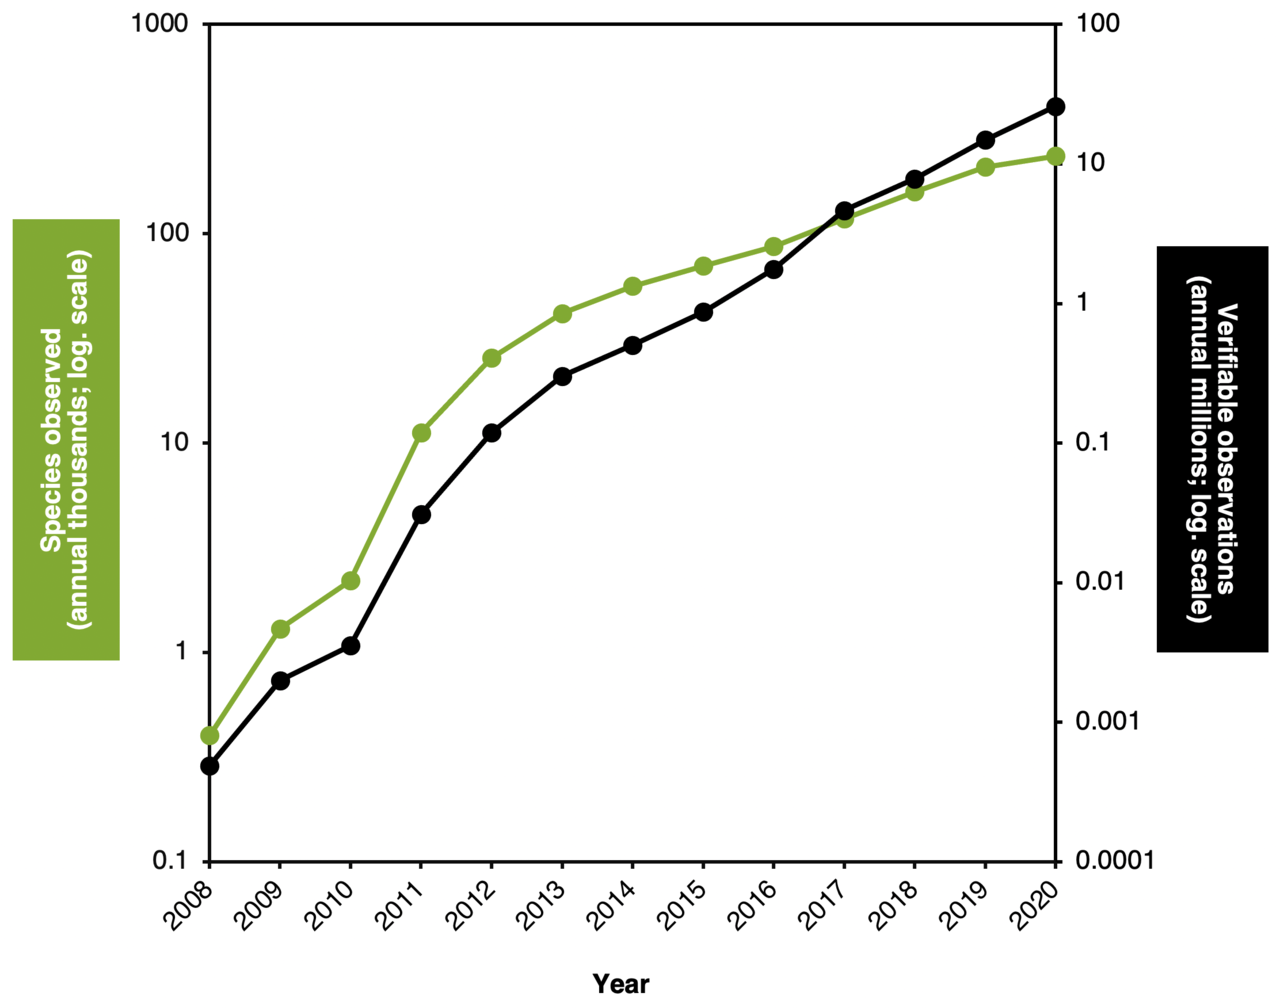
\includegraphics[scale=0.3]{inaturalist_growth.png}\\
	\tiny \href{https://commons.wikimedia.org/wiki/File:Line_graph_of_iNaturalist_activity.png}{CC BY-SA 4.0}\\
	\end{tabular}
	\end{column}
	\begin{column}{0.5\textwidth}
	\begin{tcolorbox}[title=Observation, colframe=UNBCGreen]
	There are people willing to collect field data.
	\end{tcolorbox}
	
	\begin{qmarker}
	Can citizen scientists be persuaded to collect slightly different data if they provided with a working example?
	\end{qmarker}
	\end{column}
	\end{columns}
\end{frame}

\begin{frame}
	\frametitle{I Love Moose}
	\begin{columns}
	\begin{column}{0.4\textwidth}
	\centering
	\tiny
	\textbf{Forum Questions}
	\begin{itemize}
		\item \href{https://biology.stackexchange.com/questions/108913/do-moose-usually-browse-woody-foilage-approximately-perpendicular-to-the-long-ax}{Do moose usually browse woody foilage approximately perpendicular to the long axis of the branch?}
		\item \href{https://biology.stackexchange.com/questions/107971/is-there-a-published-calibration-between-footprint-measurements-to-body-length-i}{Is there a published calibration between footprint measurements to body length in moose?}
		\item \href{https://biology.stackexchange.com/questions/107876/how-much-does-dry-moose-scat-weigh-and-vary-in-dry-weight}{How much does dry moose scat weigh and vary in dry weight?}
		\item \href{https://stats.stackexchange.com/questions/575245/how-can-i-adjust-cumulative-entropy-of-moose-observations}{How can I adjust cumulative entropy of moose observations?}
		\item \href{https://stats.stackexchange.com/questions/575100/bounds-of-integration-for-marginalizing-moose-poop-density}{Bounds of integration for marginalizing moose poop density}
	\end{itemize}
	\end{column}
	\begin{column}{0.6\textwidth}
	\begin{tabular}{cc}
	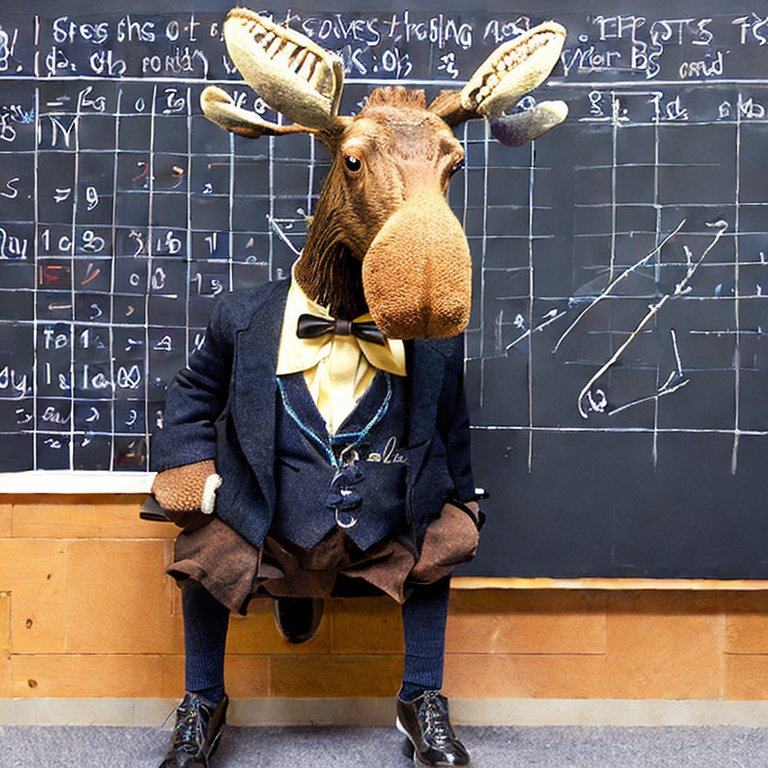
\includegraphics[scale=0.15]{moose_mathematician.jpeg} & 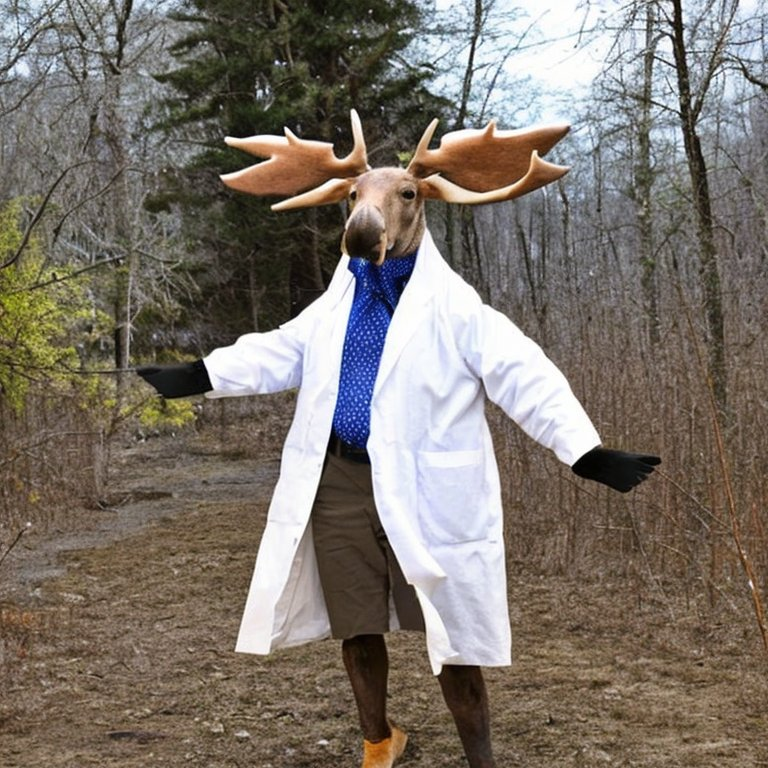
\includegraphics[scale=0.15]{moose_scientist.jpeg} \\
	\tiny \ccPublicDomain\ \href{https://stablediffusionweb.com/}{https://stablediffusionweb.com/} & \tiny \ccPublicDomain\ \href{https://stablediffusionweb.com/}{https://stablediffusionweb.com/} \\
	\end{tabular}
	\end{column}
	\end{columns}
	\begin{tabular}{cc}

\includegraphics[scale=0.4]{cvbrag.png} & 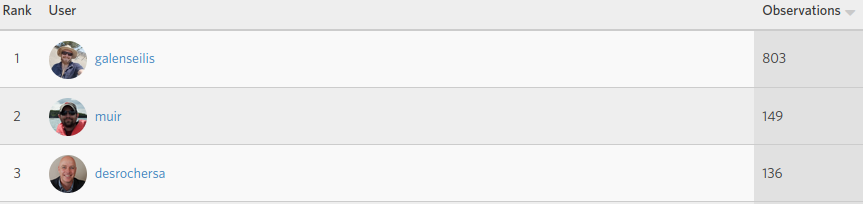
\includegraphics[scale=0.4]{leaderboard.png}\\
\tiny Fair Use & \tiny Fair Use \\
	\end{tabular}
\end{frame}

\begin{frame}
	\frametitle{From Collar to Compass}
	
	\begin{tabular}{cc}
	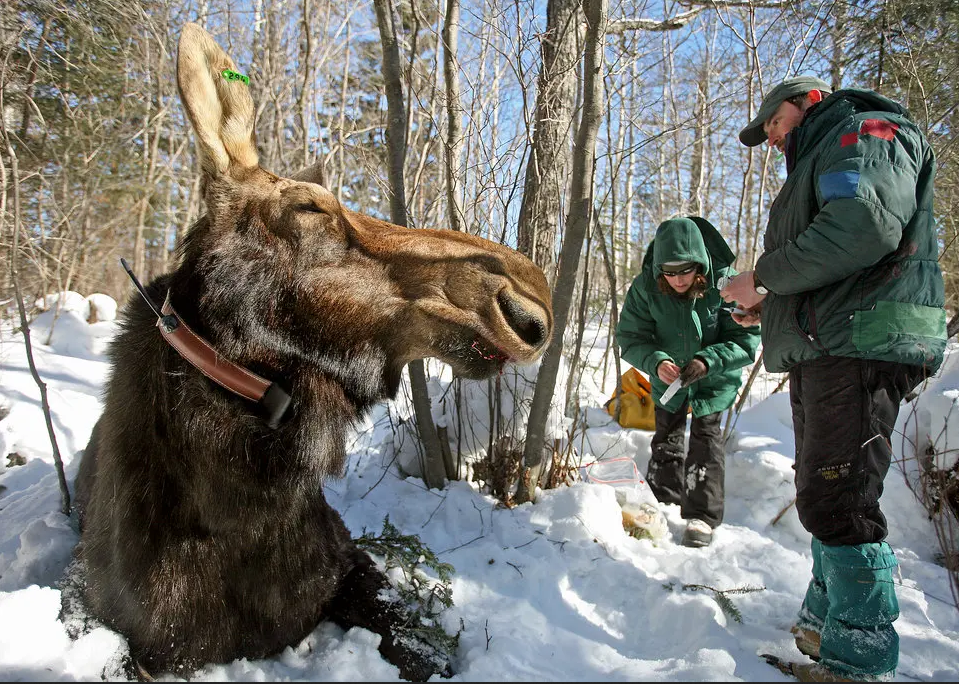
\includegraphics[scale=0.332]{moosecollar.png} & 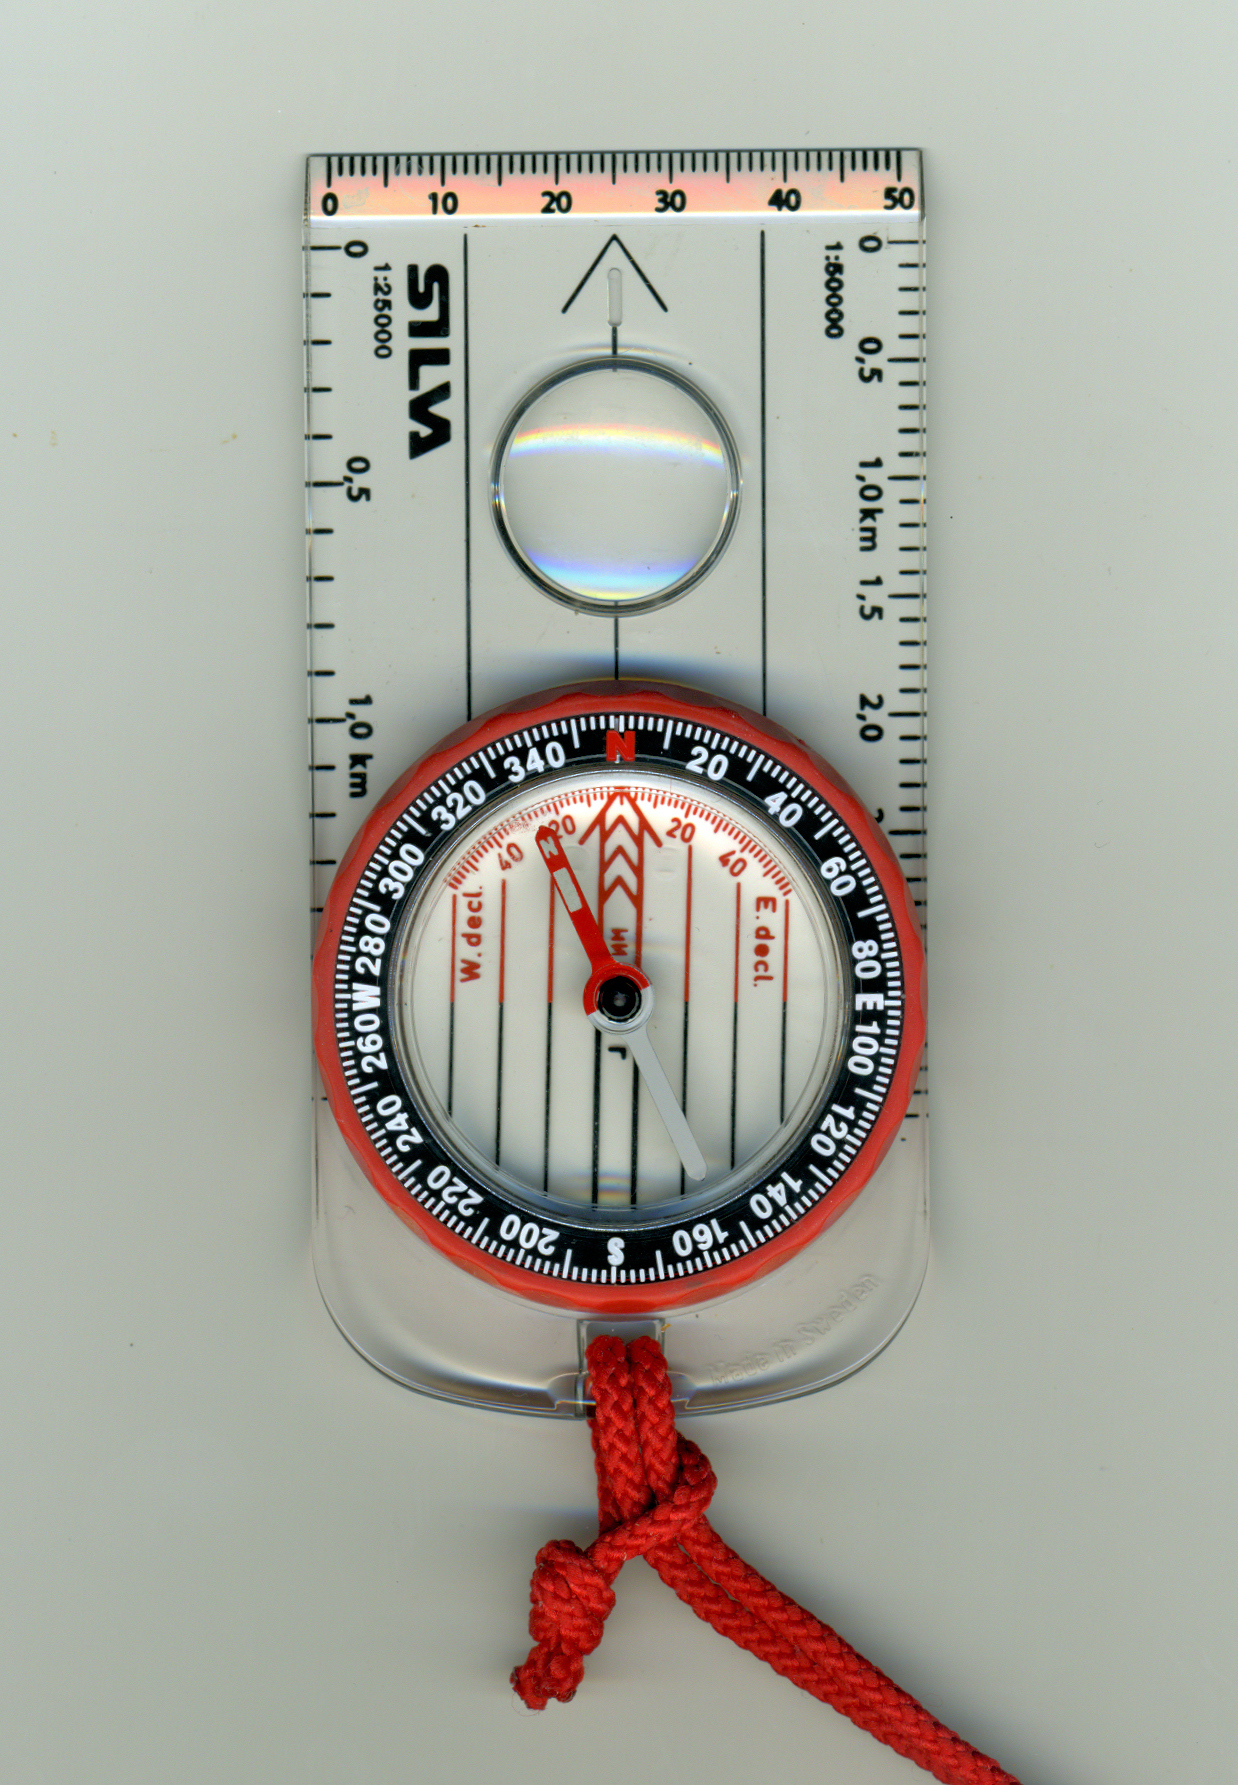
\includegraphics[scale=0.4]{compass.jpeg} \\
	\tiny \ccCopy\ Brian Peterson & \tiny \ccPublicDomain\ Public Domain \\
	\tiny Fair Use & \\
	\end{tabular}
\end{frame}

\section{Indicators}

\begin{frame}
	\frametitle{Overview}
	\begin{columns}
	\begin{column}{0.5\textwidth}
	\begin{itemize}
		\item Tracks
		\item Large snapped plants
		\item Chewed bark
		\item Chewed buds
		\item Scat
		\item Wildlife cameras
	\end{itemize}
	\end{column}
	\begin{column}{0.5\textwidth}
	\begin{tcolorbox}[title=Definition, colframe=UNBCGreen]
	An an observation is a \textbf{weak indicator} of orientation if it is compatible with multiple orientations.
	\end{tcolorbox}
	\begin{tcolorbox}[title=Definition, colframe=UNBCGreen]
	An an observation is a \textbf{local indicator} of orientation if it describes orientation at a small and particular place.
	\end{tcolorbox}
	\begin{cmarker}
	Partial pooling may allow non-local estimates of orientation.
	\end{cmarker}
	\end{column}
	\end{columns}
\end{frame}

\begin{frame}
	\frametitle{Tracks}
	\begin{tabular}{ccc}
	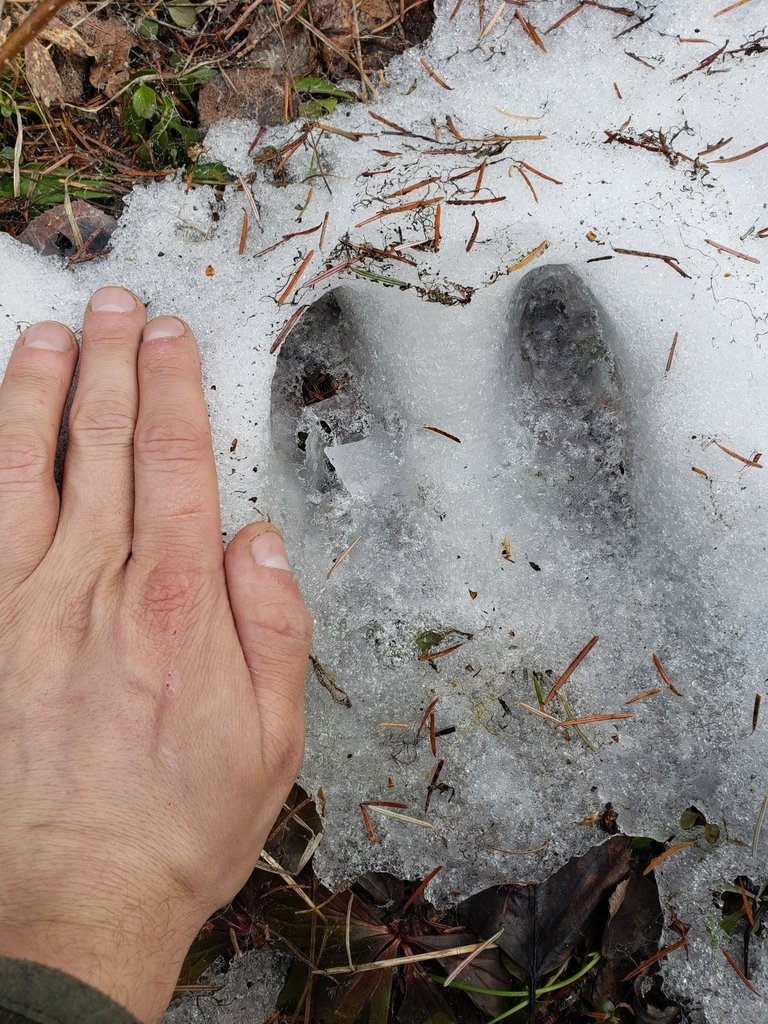
\includegraphics[scale=0.16]{snowtrack.jpeg} & 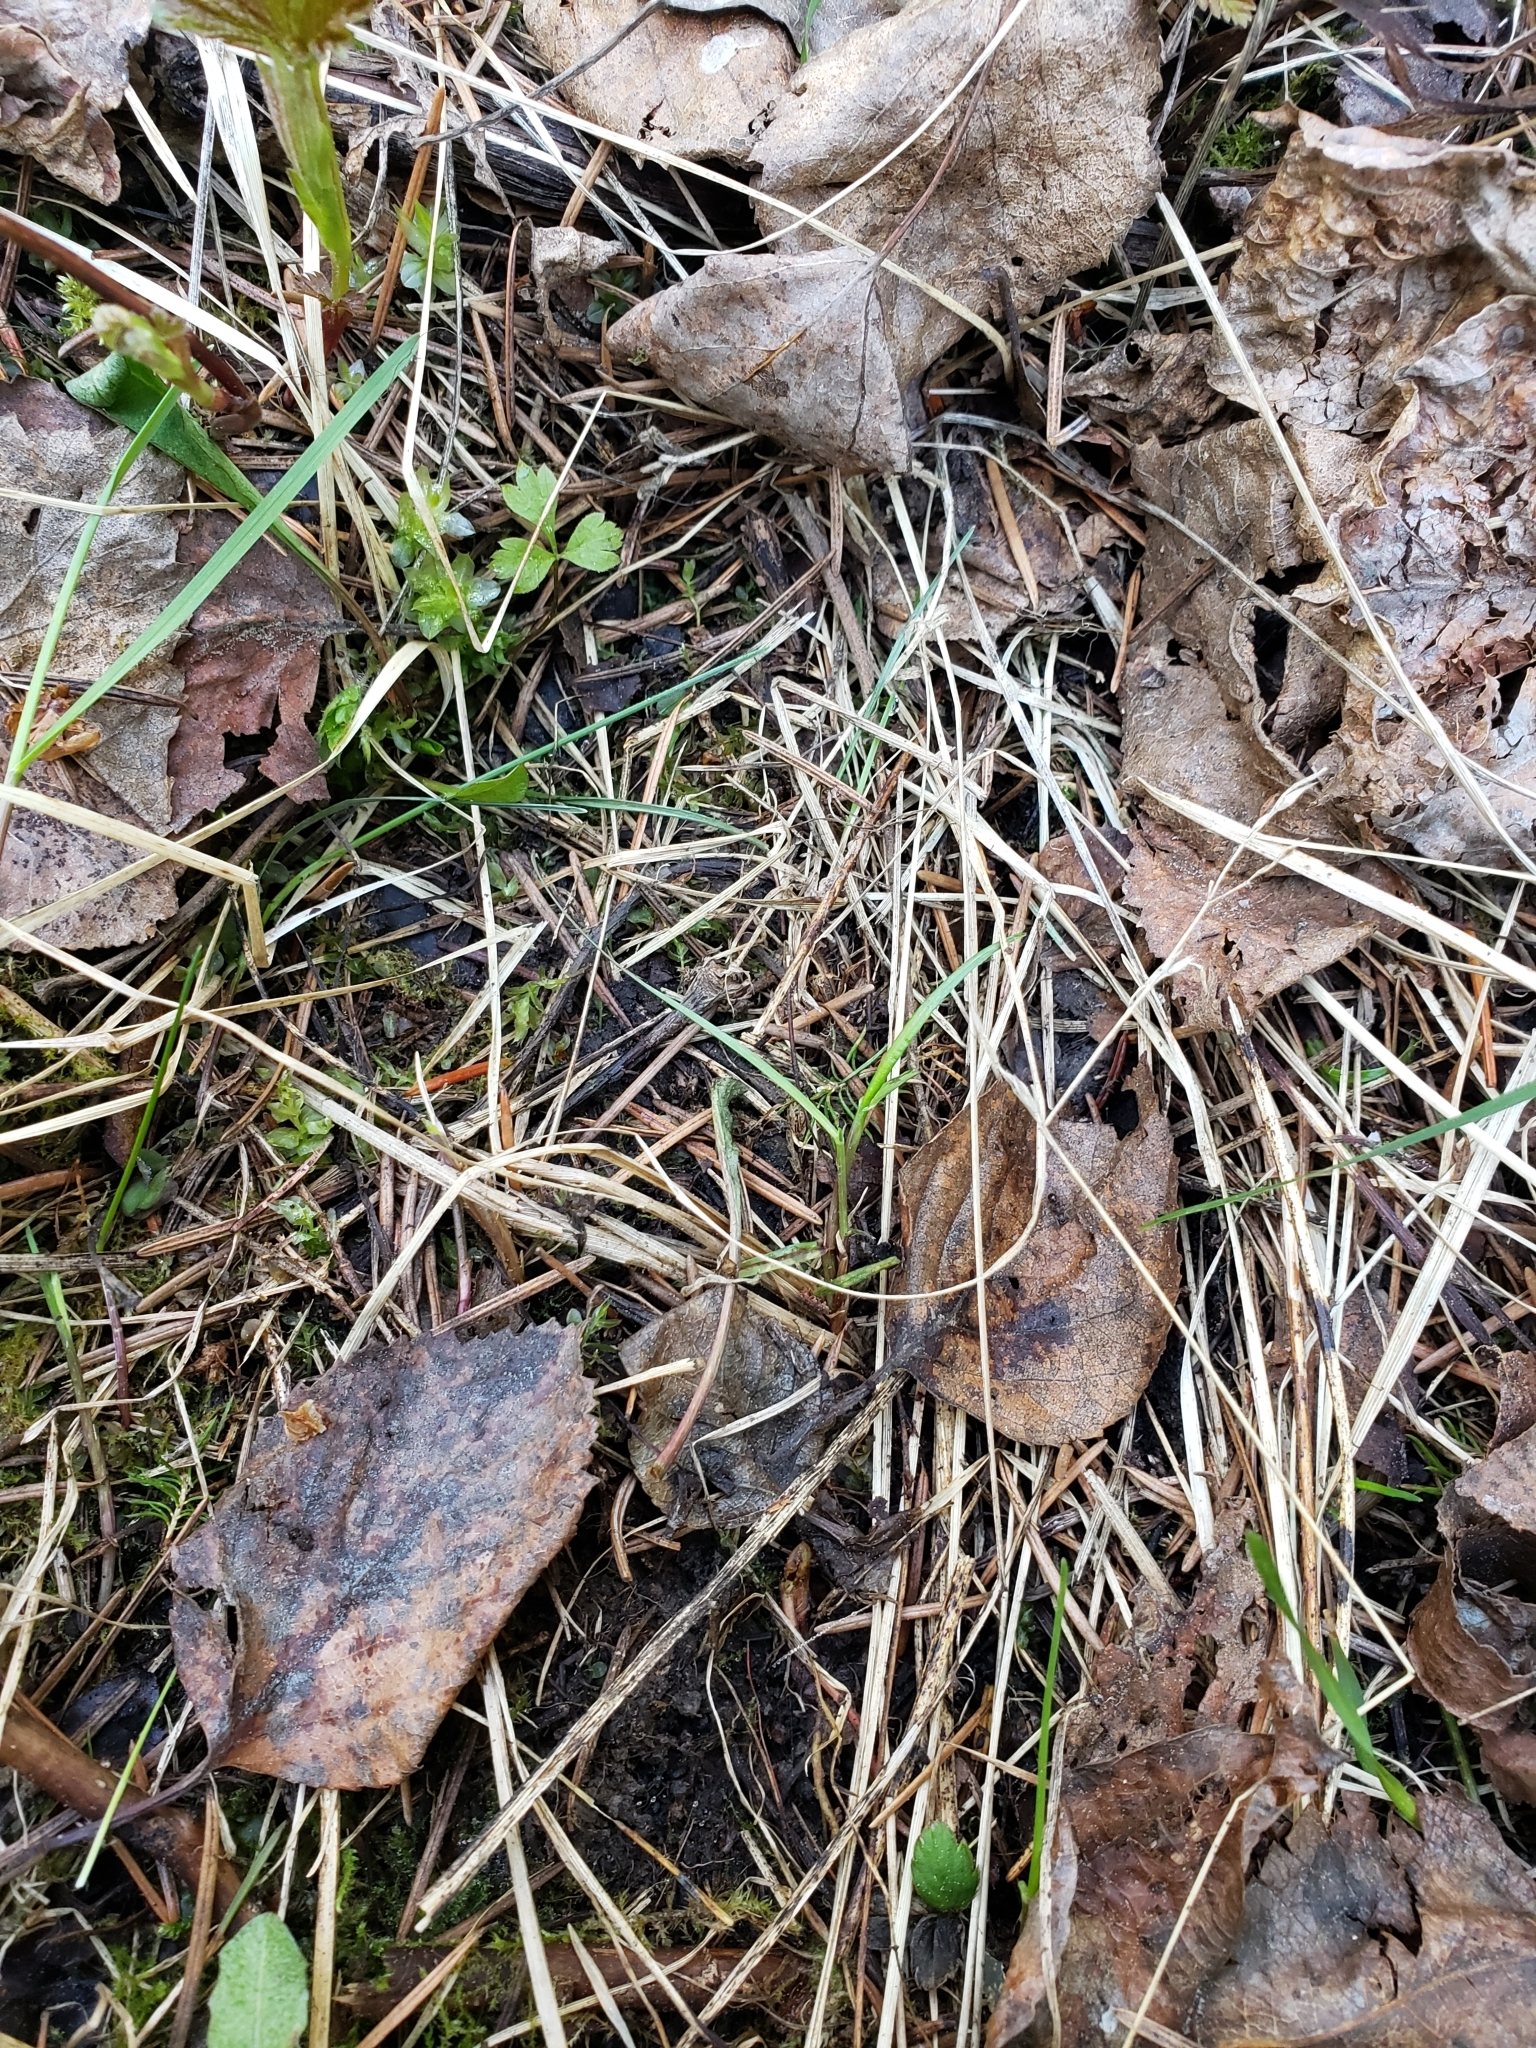
\includegraphics[scale=0.08]{trackingrass.jpeg} & 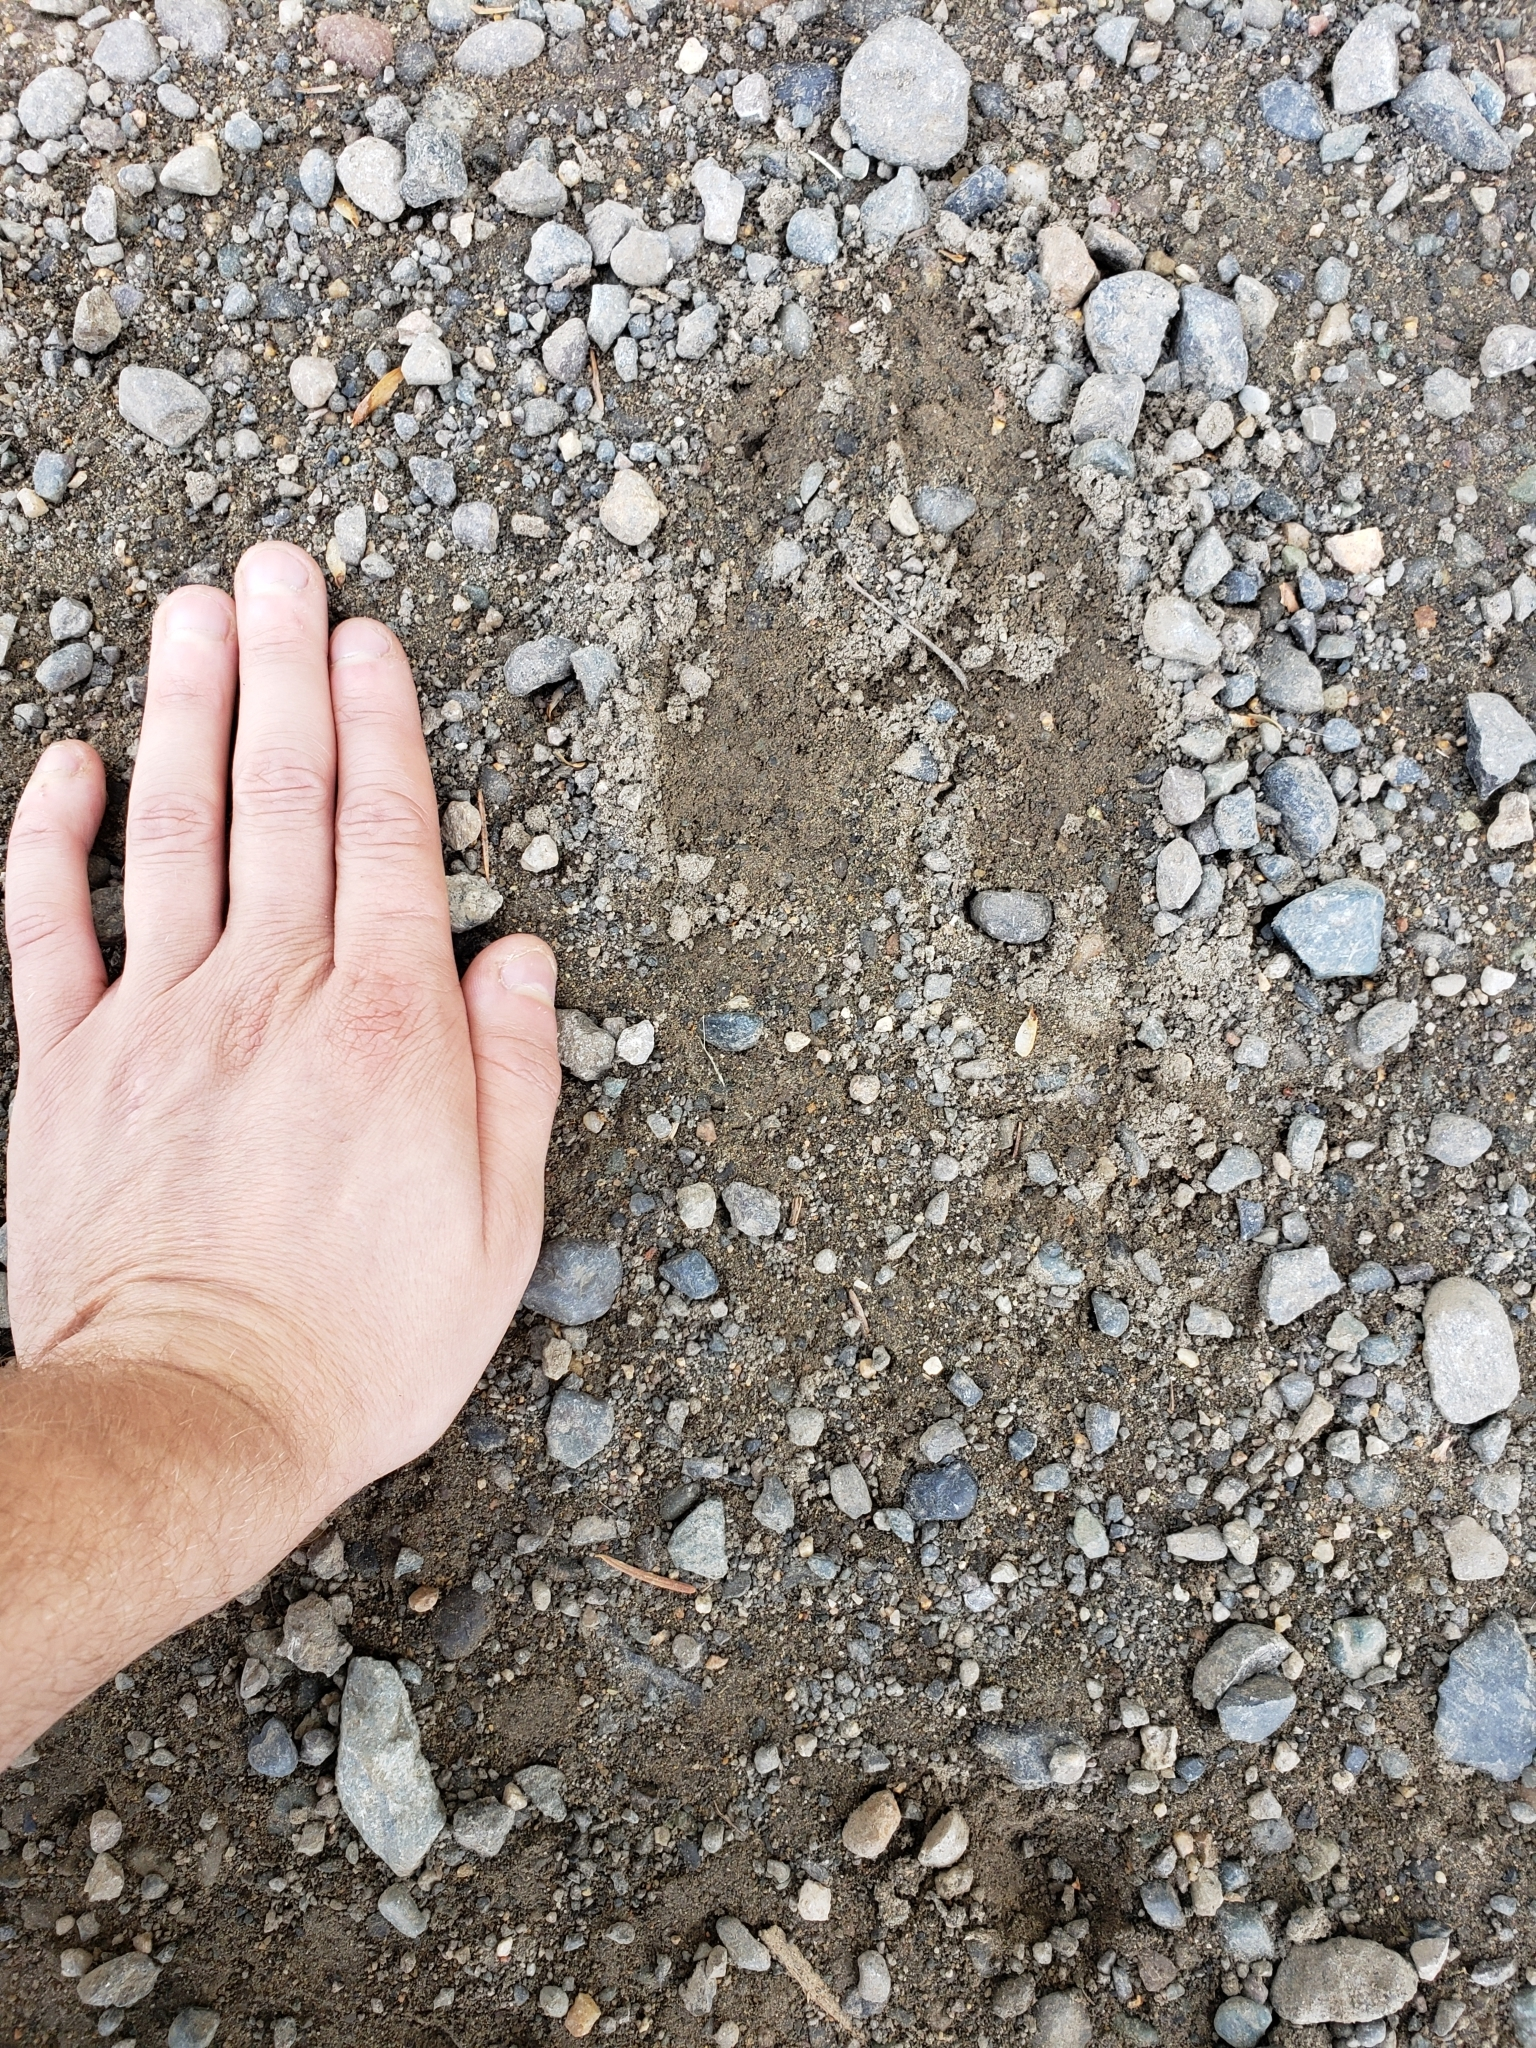
\includegraphics[scale=0.08]{trackonroad.jpeg} \\
	\tiny \ccCopy\ Galen Seilis & \tiny \ccCopy\ Galen Seilis & \tiny \ccCopy\ Galen Seilis \\
	\end{tabular}
\end{frame}

\begin{frame}
	\frametitle{Large Snapped Plants}
	\centering
	\begin{tabular}{cc}
	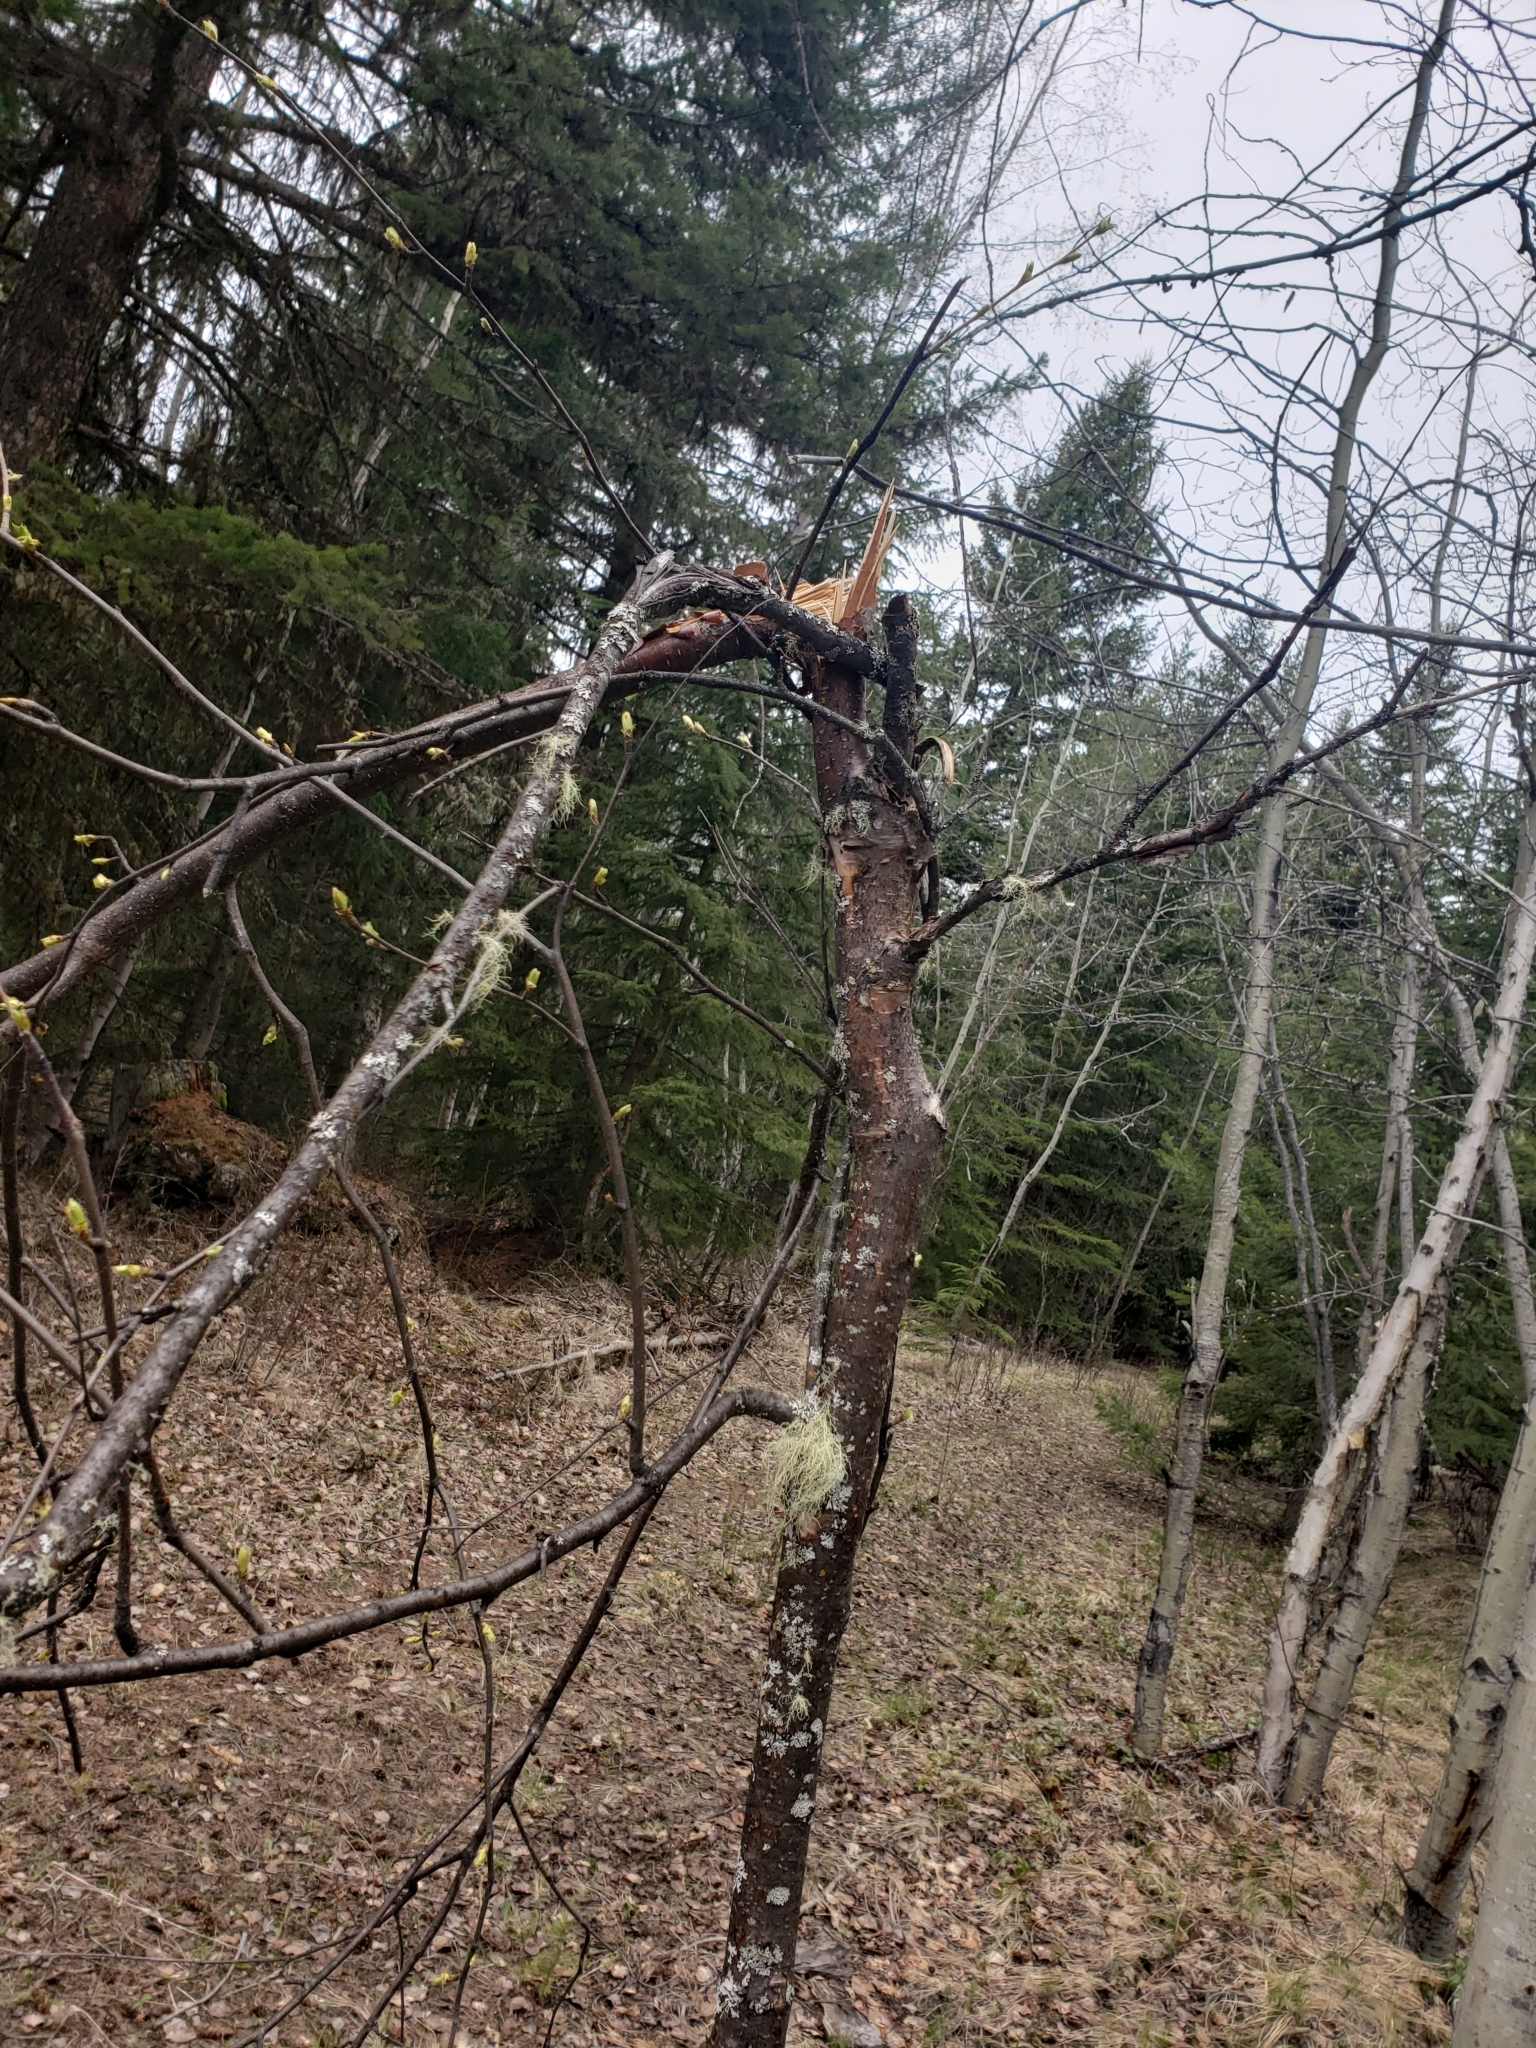
\includegraphics[scale=0.09]{brokentree.jpeg} & 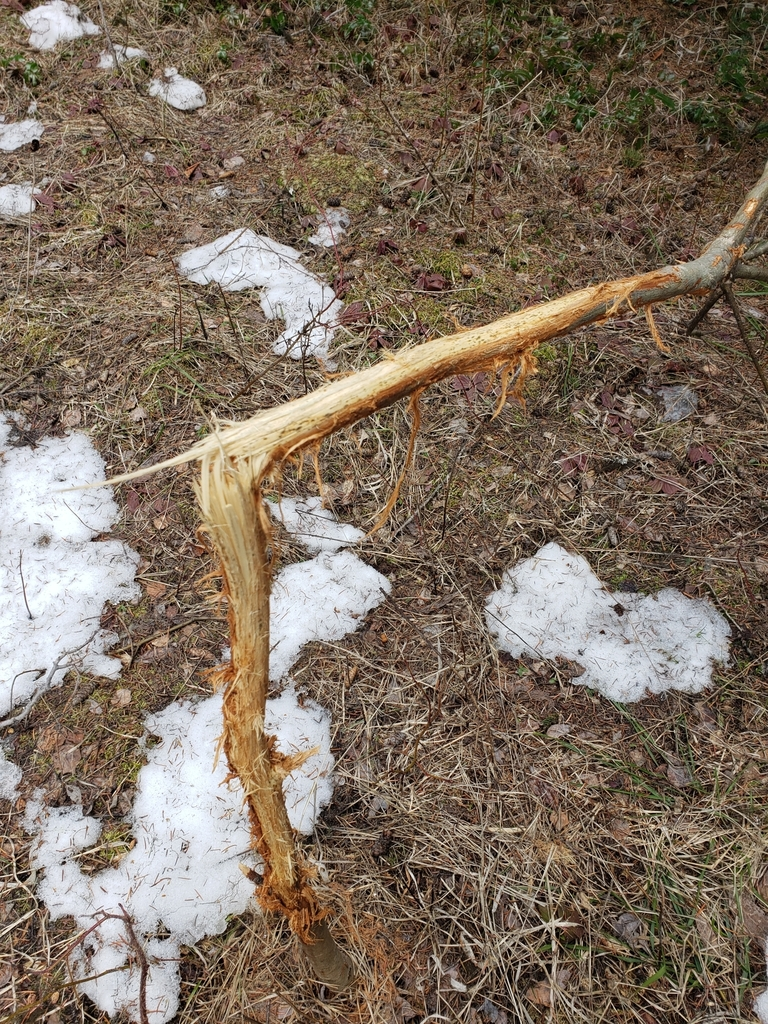
\includegraphics[scale=0.18]{brokenchewed.jpeg} \\
	\tiny \ccCopy\ Galen Seilis & \tiny \ccCopy\ Galen Seilis \\
	\end{tabular}
\end{frame}

\begin{frame}
	\frametitle{Chewed Bark}
	
	\begin{columns}
	\begin{column}{0.5\textwidth}
	\begin{tabular}{c}
	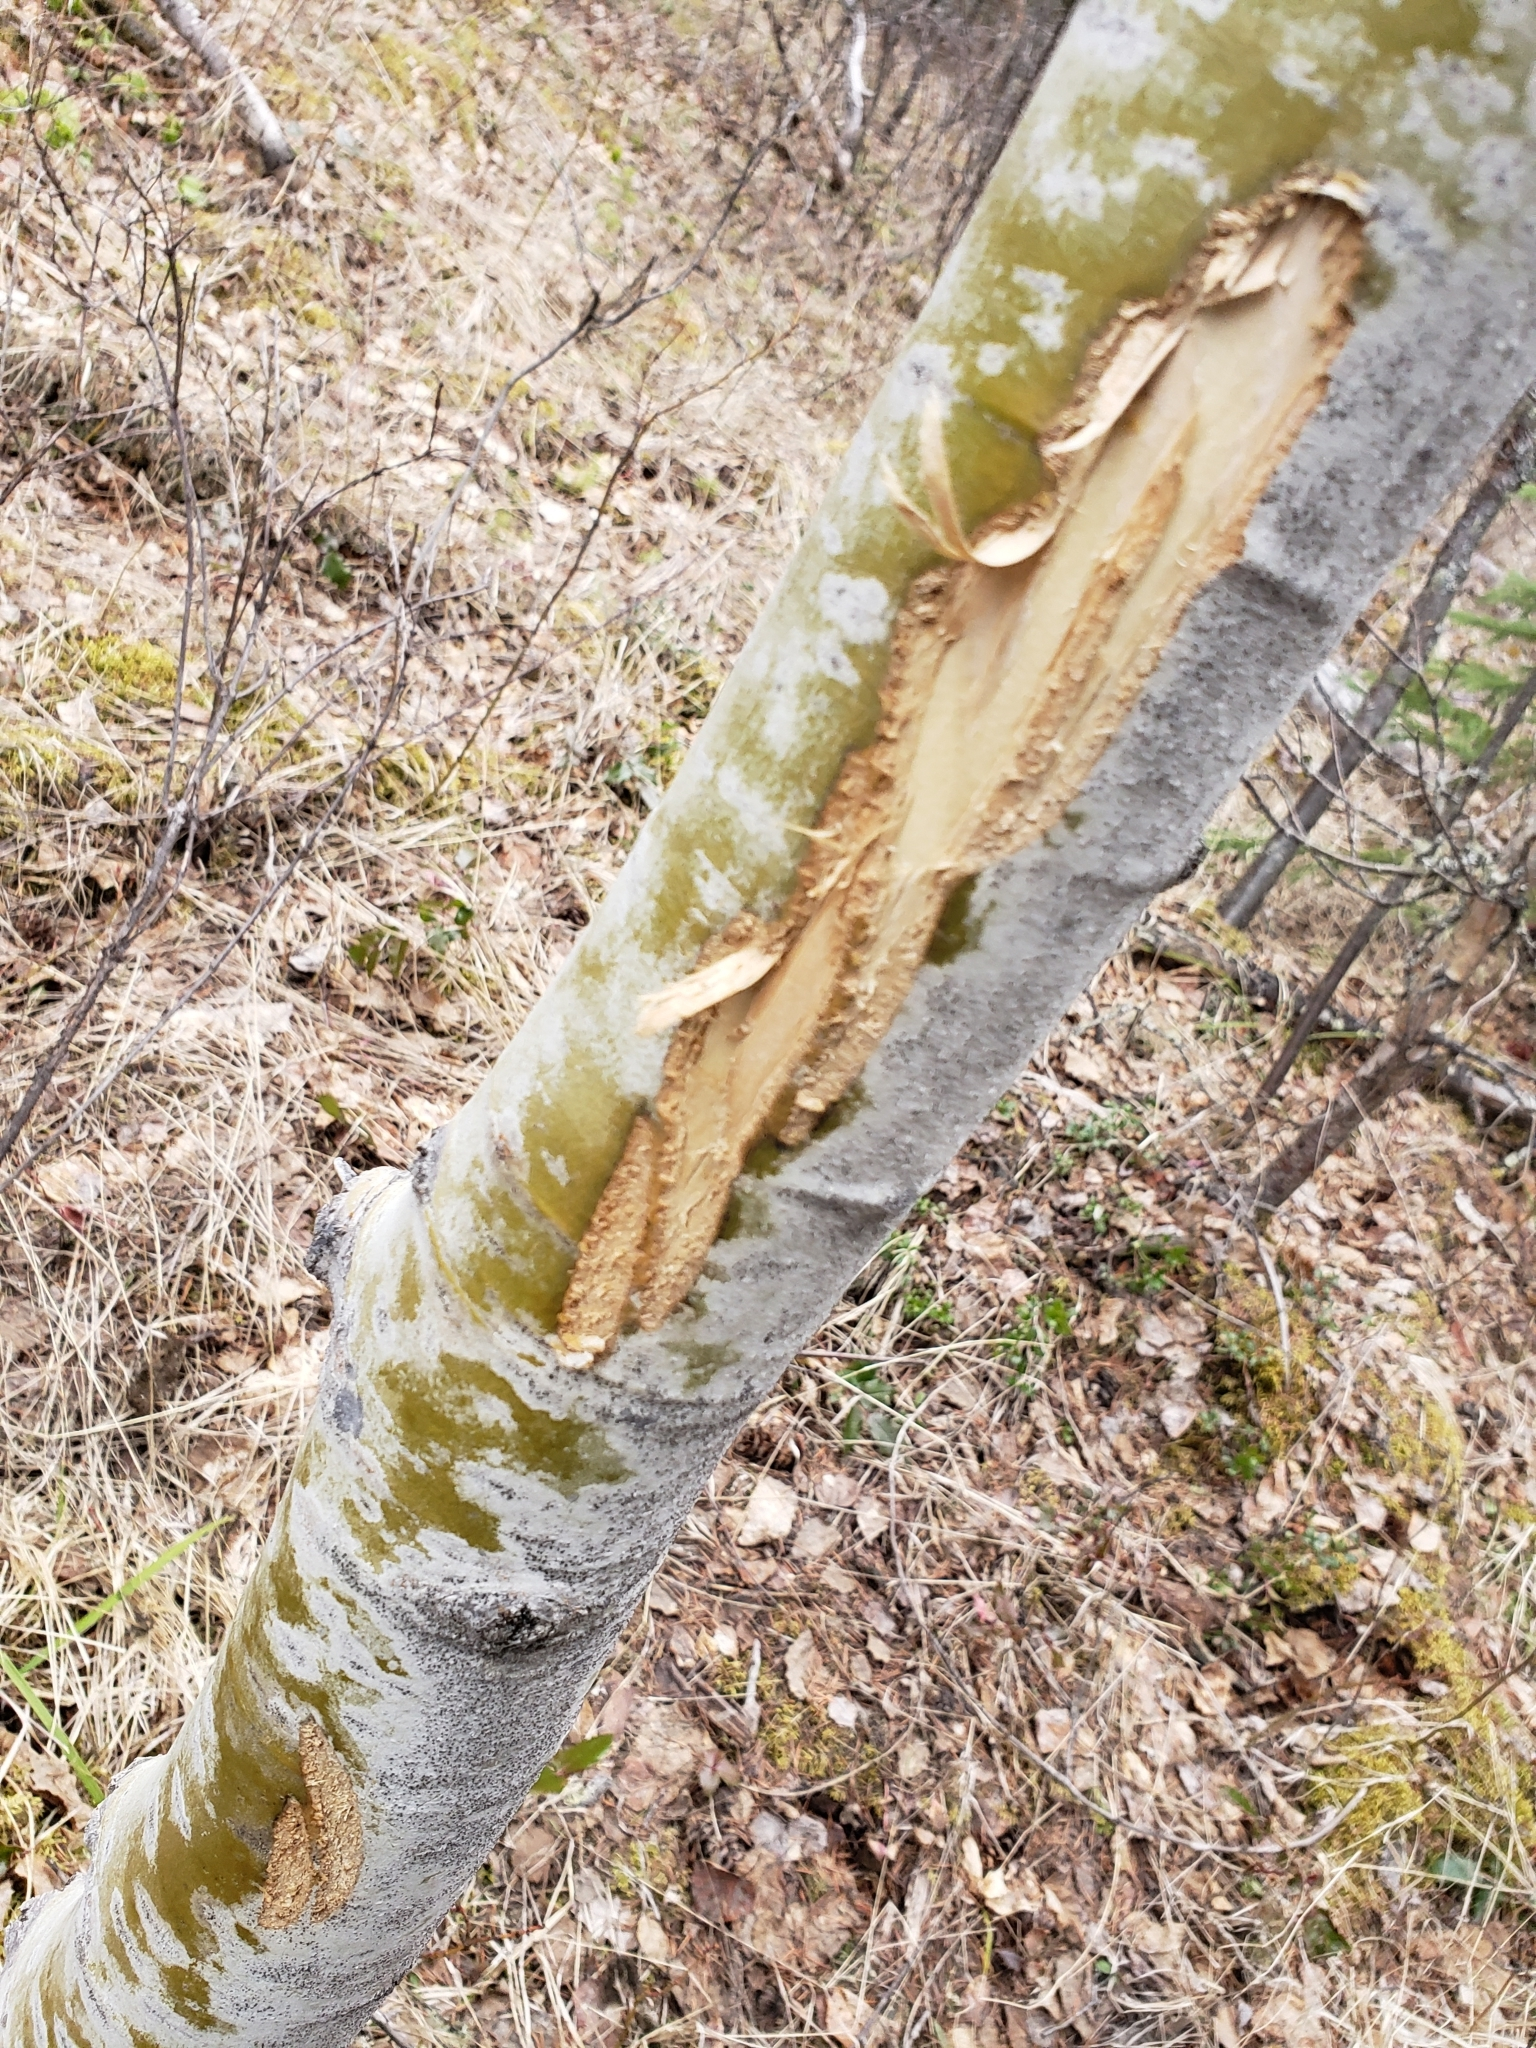
\includegraphics[scale=0.09]{chewbark.jpeg} \\
	\tiny \ccCopy\ Galen Seilis \\
	\end{tabular}
	\end{column}
	\begin{column}{0.5\textwidth}
	\begin{xmarker}
	\begin{tabular}{c}
	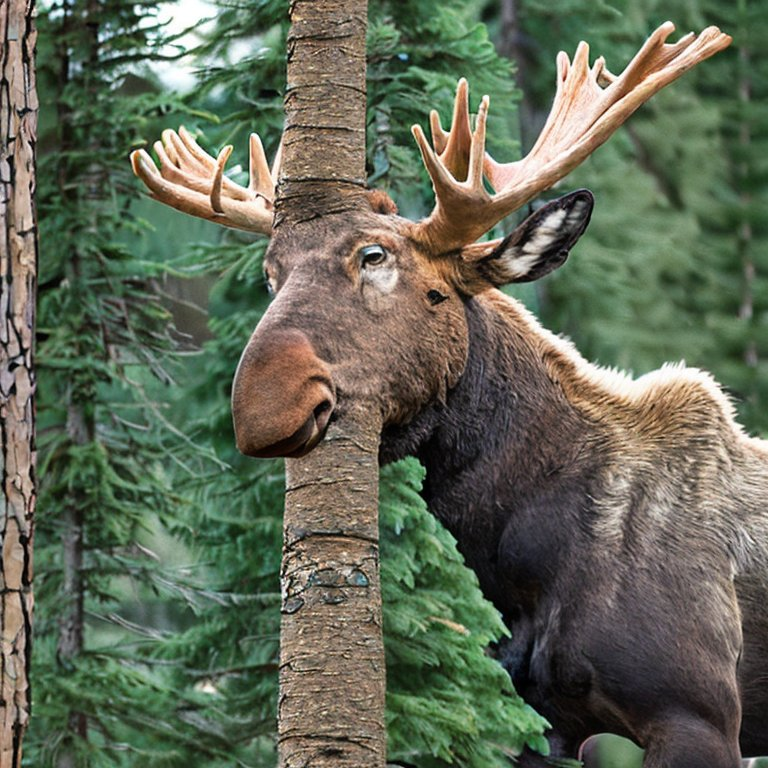
\includegraphics[scale=0.2]{moose_through_tree.jpg} \\
	\tiny \ccPublicDomain\ \href{https://stablediffusionweb.com/}{https://stablediffusionweb.com/} \\
	\end{tabular}
	\end{xmarker}
	\end{column}
	\end{columns}
\end{frame}

\begin{frame}
	\frametitle{Chewed Buds}
	
	\begin{columns}
	\begin{column}{0.4\textwidth}
	\begin{tabular}{c}
	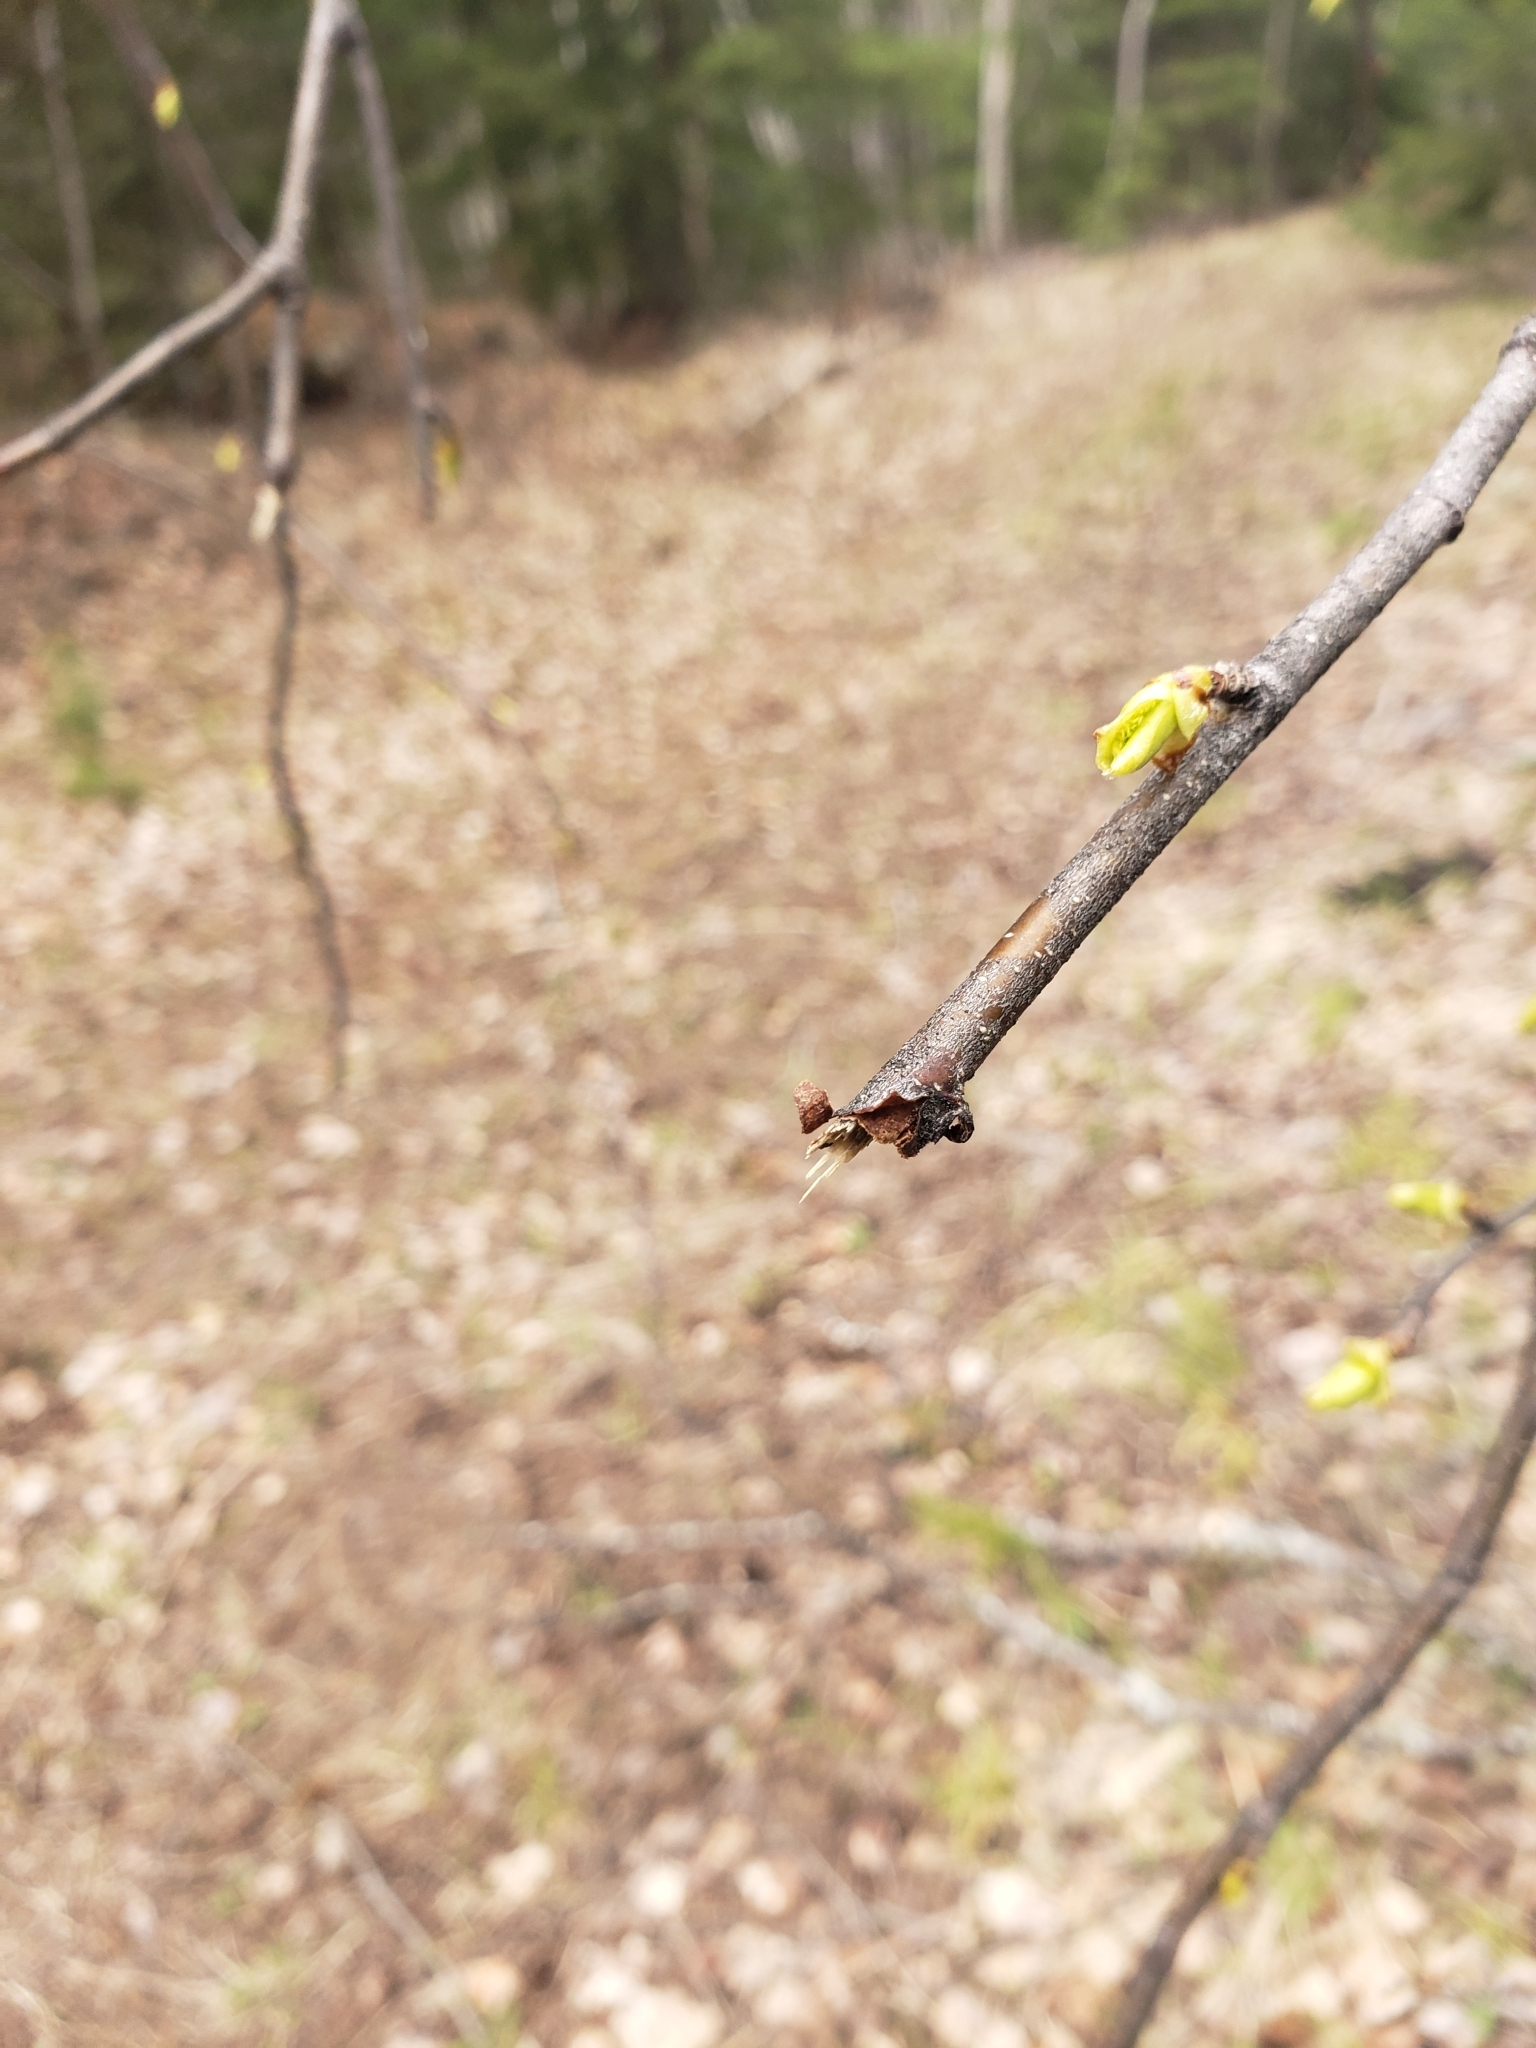
\includegraphics[scale=0.09]{chewedbud.jpeg} \\
	\tiny \ccCopy\ Galen Seilis \\
	\end{tabular}
	\end{column}
	\begin{column}{0.6\textwidth}
	\begin{imarker}
	This type of observation can be especially weak.
	\end{imarker}
	\begin{tabular}{cc}
	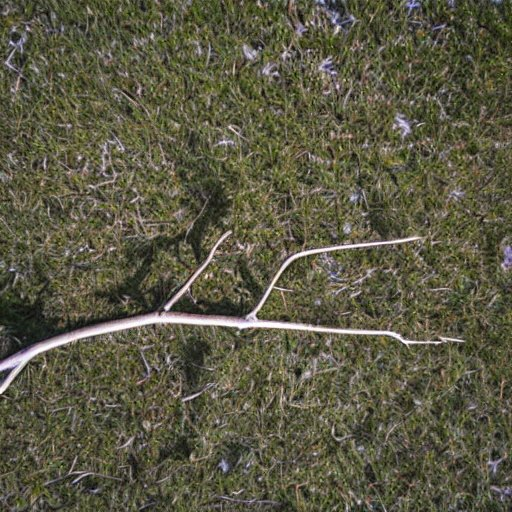
\includegraphics[scale=0.2]{branch.jpeg} & 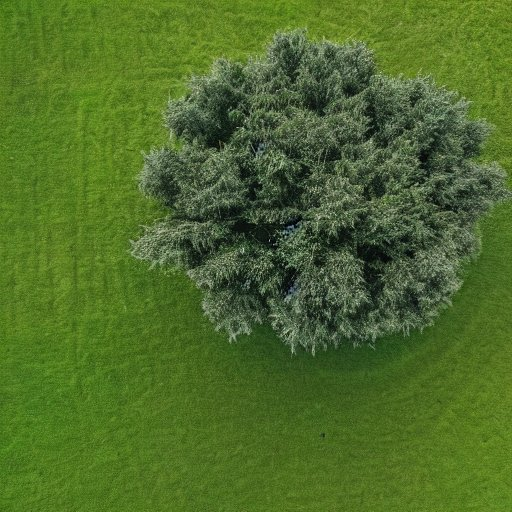
\includegraphics[scale=0.2]{bushtopdown.jpeg} \\
	\tiny \ccPublicDomain\ \href{https://stablediffusionweb.com/}{https://stablediffusionweb.com/} & \tiny \ccPublicDomain\ \href{https://stablediffusionweb.com/}{https://stablediffusionweb.com/} \\
	\end{tabular}
	\end{column}
	\end{columns}
\end{frame}

\begin{frame}
	\frametitle{Scat}
	\begin{tabular}{ccc}
	Pellet & Plopette & Plop \\
	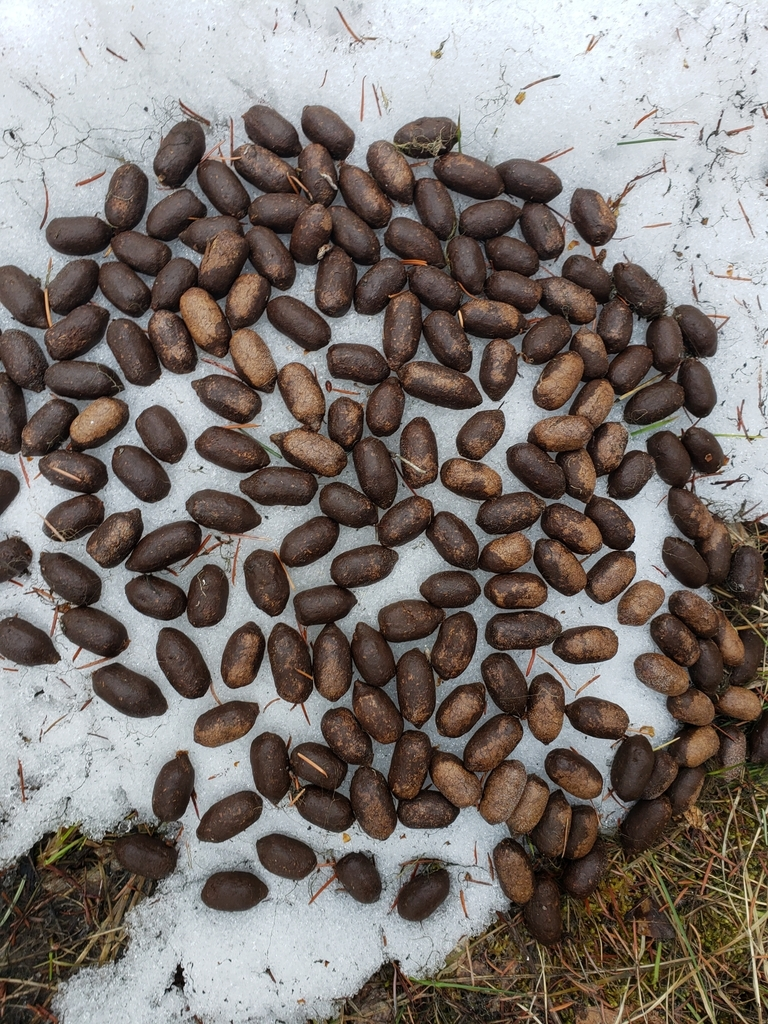
\includegraphics[scale=0.16]{scatsnow.jpeg} & 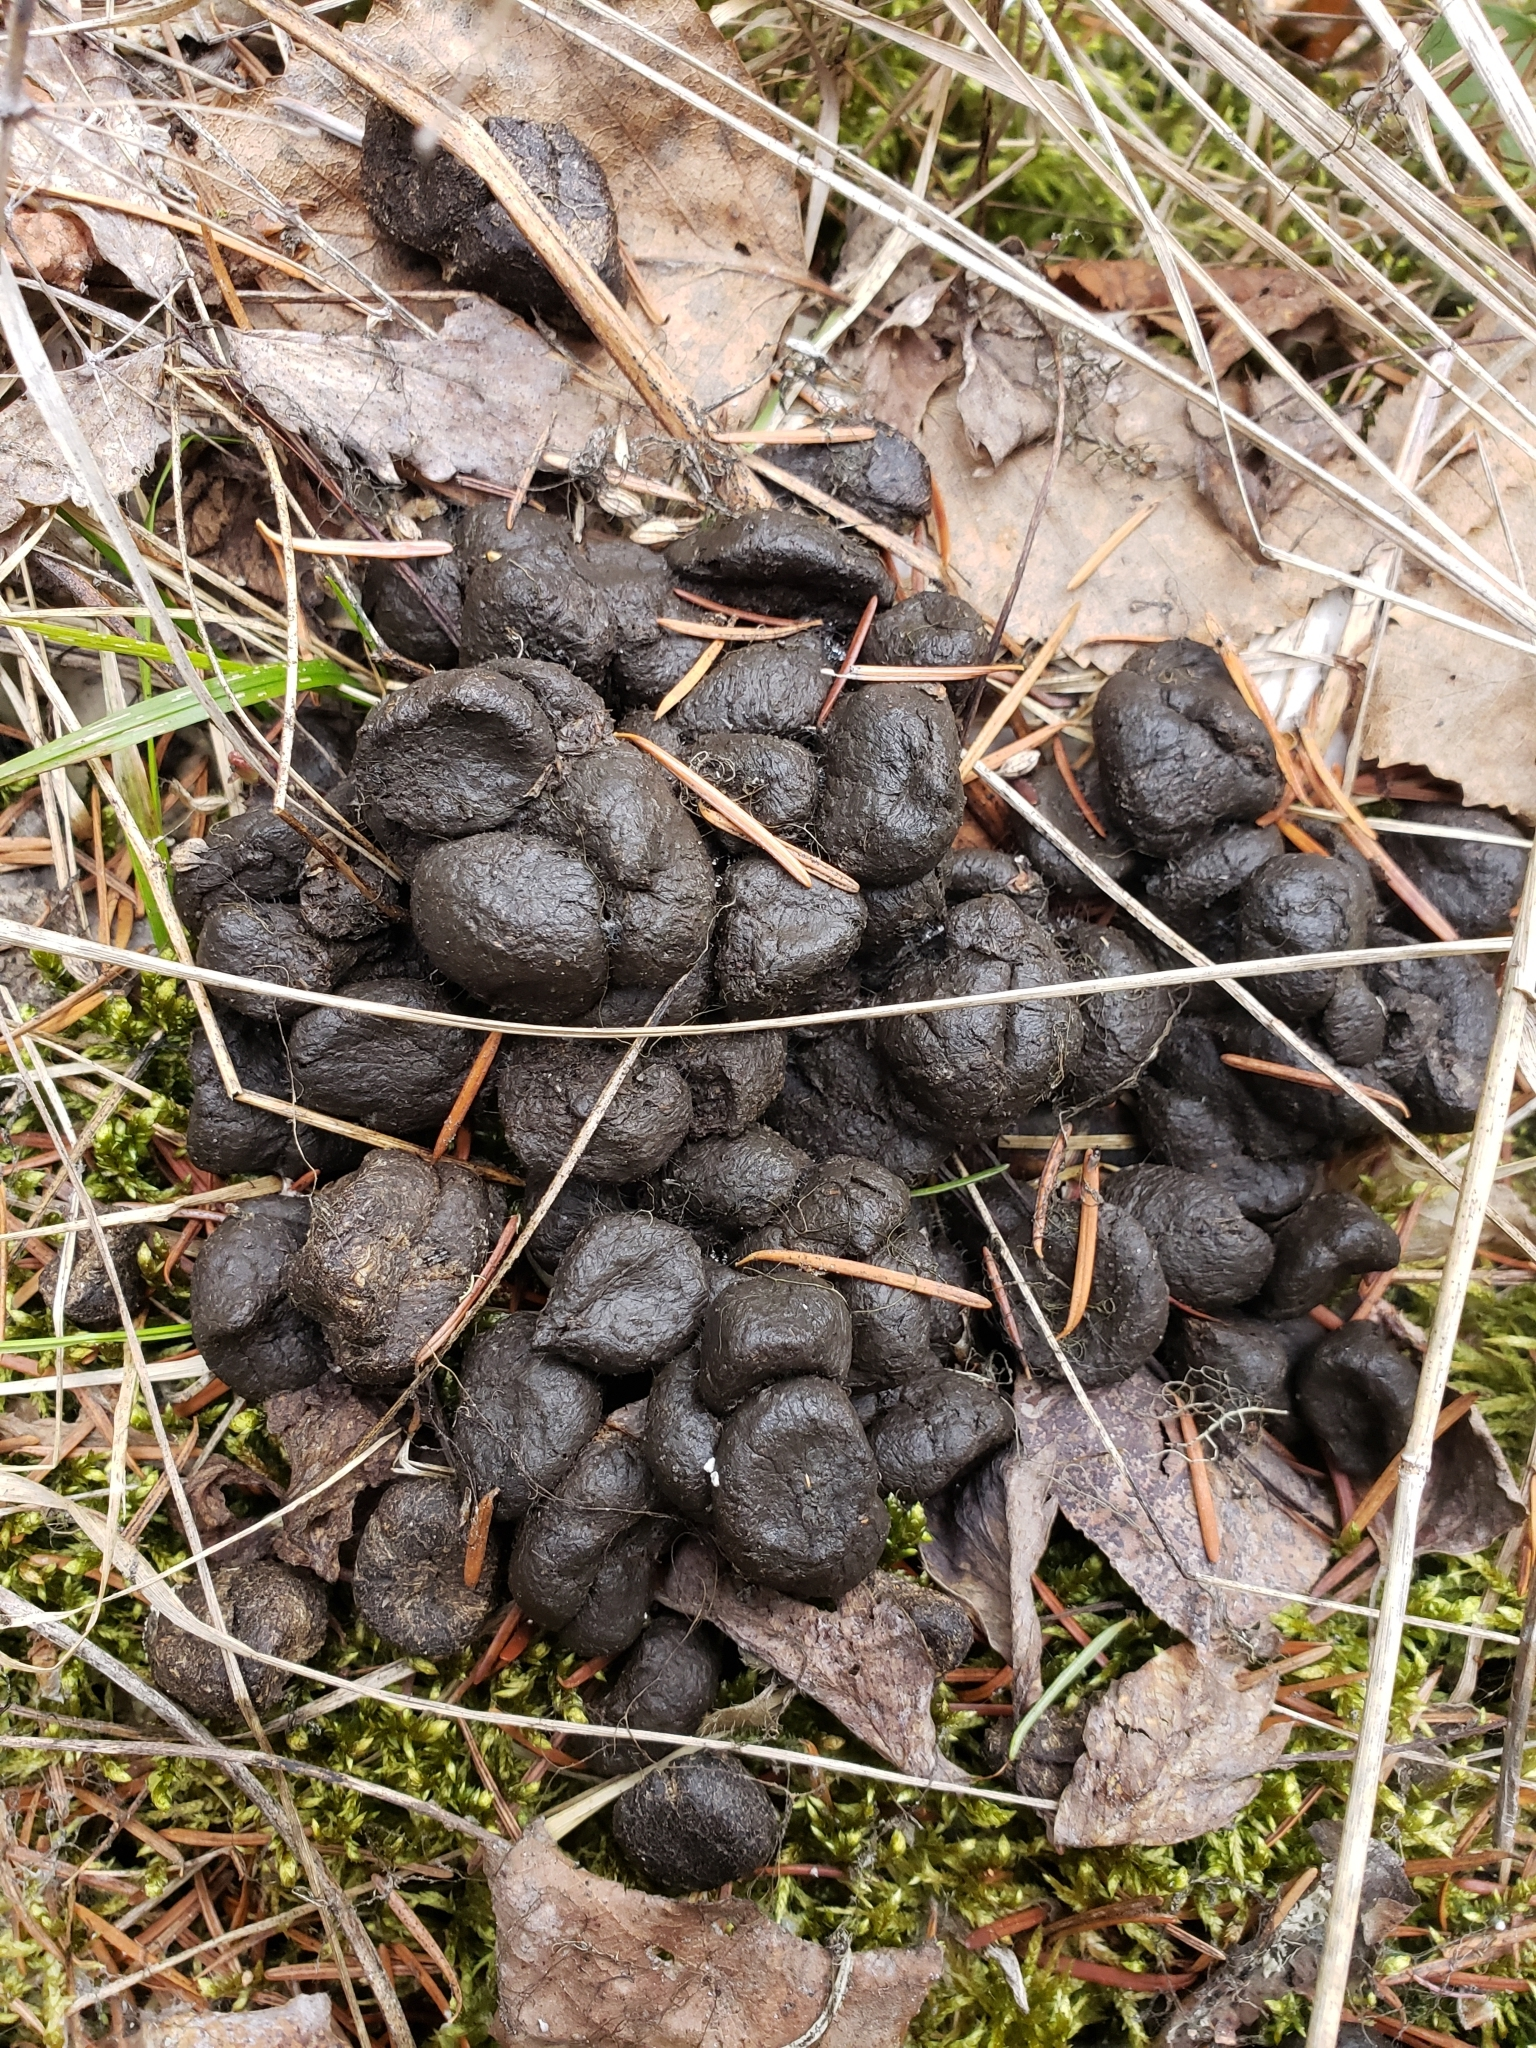
\includegraphics[scale=0.08]{ploplette.jpeg} & 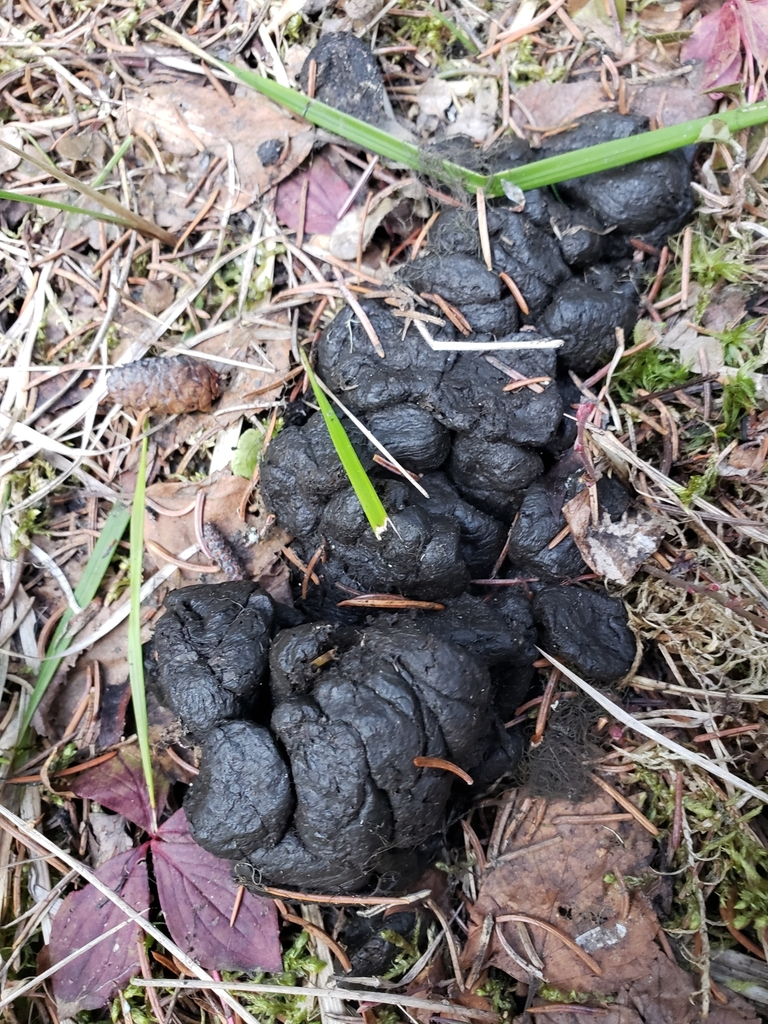
\includegraphics[scale=0.16]{plopscat.jpeg} \\
	\tiny \ccCopy\ Galen Seilis & \tiny \ccCopy\ Galen Seilis & \tiny \ccCopy\ Galen Seilis \\
	\end{tabular}
\end{frame}

\begin{frame}
	\frametitle{Wildlife Cameras}
	\begin{columns}
	\begin{column}{0.5\textwidth}
	\begin{tabular}{c}
	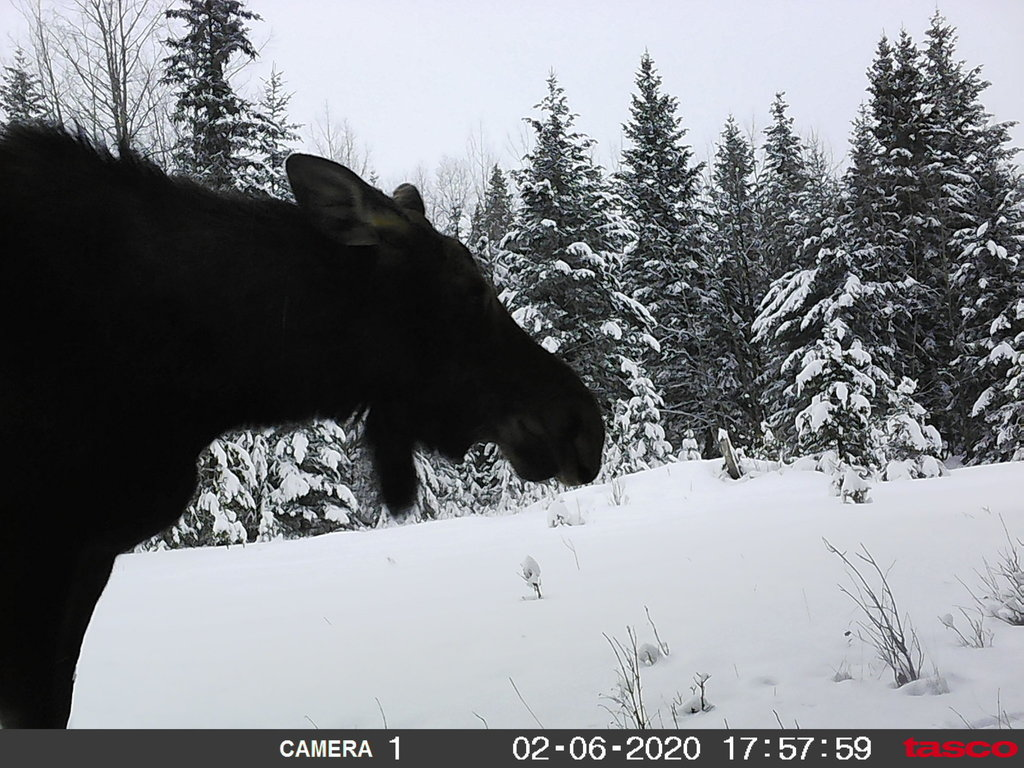
\includegraphics[scale=0.2]{wildlife_cam_example2.jpeg} \\
	\tiny \ccCopy\ Galen Seilis \\
	\end{tabular}
	\end{column}
	\begin{column}{0.5\textwidth}
	\begin{tabular}{c}
	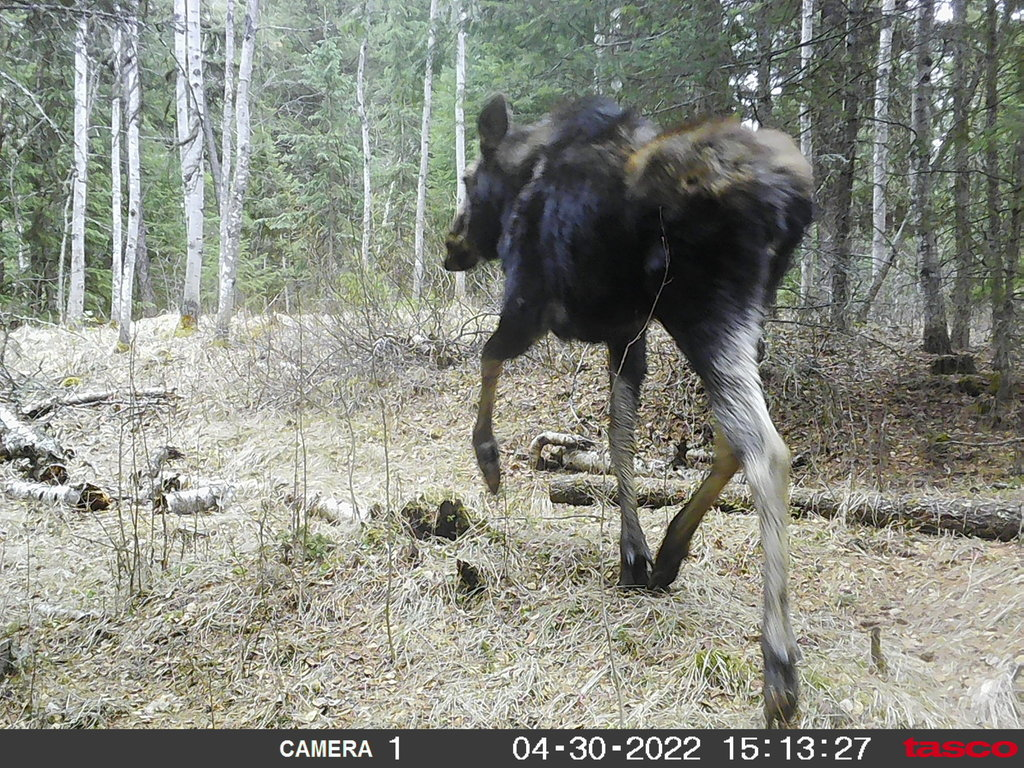
\includegraphics[scale=0.2]{wildlife_cam_example.jpeg} \\
	\tiny \ccCopy\ Galen Seilis \\
	\end{tabular}
	\end{column}
	\end{columns}
\end{frame}

\section{Covariates \& Confounds}

\begin{frame}
	\frametitle{Overview}	
	\begin{columns}
	\begin{column}{0.5\textwidth}
	\begin{itemize}
		\item Wind
		\item Slope
		\item Aspect
		\item Debris
		\item Vegetation
		\item Sampling Intensity
		\item Animal disturbance
		\item Snow melt
	\end{itemize}
	\end{column}
	\begin{column}{0.5\textwidth}
	\begin{qmarker}
	Would building a structural model accounting for some or all of these variables improve model performance?
	\end{qmarker}
	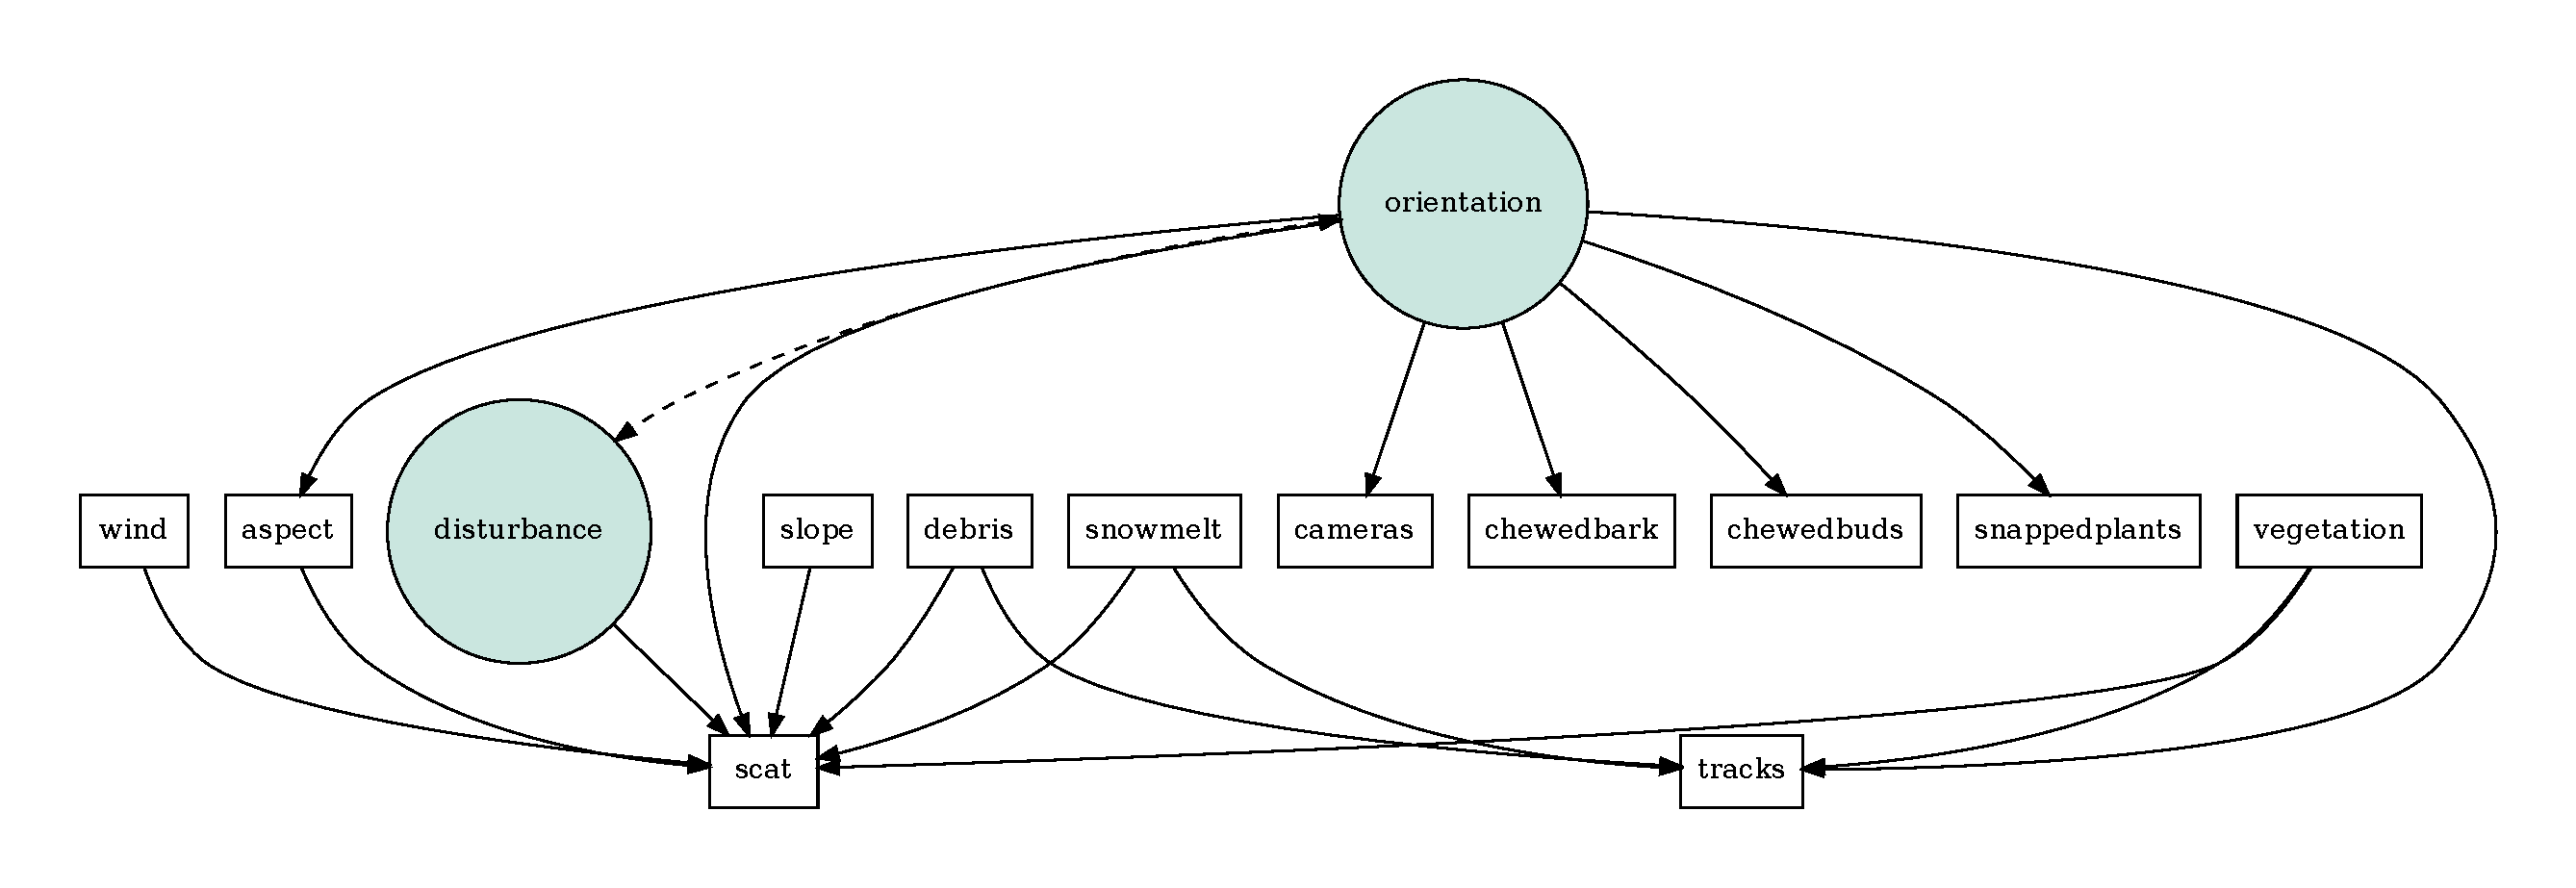
\includegraphics[scale=0.15]{sem.pdf}
	\begin{imarker}
	Collecting more data requires additional effort.
	\end{imarker}
	\end{column}
	\end{columns}
\end{frame}

\section{Modelling Approaches}

\begin{frame}
	\frametitle{Bayesian Inference}	
	\begin{columns}
	\begin{column}{0.5\textwidth}
	\begin{cmarker}
	\begin{itemize}
	\item Include prior information
	\item Can study model-implied covariances
	\item Incorporates epistemic and aleatory uncertainty
	\item Degrees of freedom are not a problem
	\item Parameters are random variables
	\end{itemize}
	\end{cmarker}
	\tiny Reporting: \href{https://www.nature.com/articles/s41562-021-01177-7}{Kruschke 2021, \textit{Bayesian Analysis Reporting Guidelines}}.\\
	
	\tiny Course: \href{https://www.youtube.com/playlist?list=PLDcUM9US4XdMROZ57-OIRtIK0aOynbgZN}{Richard McElreath, \textit{Statistical Rethinking} 2022}.
	\end{column}
	\begin{column}{0.5\textwidth}
	\begin{tmarker}[title=Circular Distributions]
	\begin{itemize}
		\item von Mises ($\mu \in \mathbb{R}$, $\kappa \in (0, \infty)$)
		\item Uniform ($-\pi \leq a < b \leq \pi$)
		\item Truncated normal ($\mu \in \mathbb{R}$, $\sigma >0$, $-\pi \leq a < b \leq \pi$)
		\item Mixtures (any)
	\end{itemize}
	\tcbline
	\begin{itemize}
		\item Bounded distributions can be used to limit possibility.
	\end{itemize}
	\end{tmarker}
	\end{column}
	\end{columns}
\end{frame}

\begin{frame}
	\frametitle{Mixed Effects / Multilevel / Hierarchical Models}
	\begin{cmarker}
	\begin{itemize}
		\item Account for types of measurements
		\item Account for spatial proximity of observations
		\item Allows estimate of both local and global effects
	\end{itemize}
	\end{cmarker}
	
	\begin{tmarker}
	With model $f(\vec x; \vec \theta)$ we may take any $\theta_j$ and replace it with
	$$\theta_j := \gamma + \sum_{i=1}^k \beta_i \mathbb{I}_i$$
	\end{tmarker}
\end{frame}

\section{Collaboration}

\begin{frame}
	\frametitle{Collaboration}
	\begin{columns}
	\begin{column}{0.5\textwidth}
	\begin{xmarker}
	I don't have the time to do data collection, or much literature review / writing about moose.
	\end{xmarker}
	\begin{cmarker}
	I'm willing to take on the statistical analysis.
	\begin{itemize}
		\item EDA
		\item Modelling
		\item Figures
	\end{itemize}
	\end{cmarker}
	\end{column}
	\begin{column}{0.5\textwidth}
	\begin{cmarker}
	I don't need to be the first author if someone wants to take this project on.
	\end{cmarker}
	\begin{imarker}
	Bayesian inference is mainstream, but not understood or accepted everywhere.
	\end{imarker}
	\end{column}
	\end{columns}
\end{frame}

\end{document}
